        %%******************************************%%
        %%                                          %%
        %%        Modello di tesi di laurea         %%
        %%            di Andrea Giraldin            %%
        %%                                          %%
        %%             2 novembre 2012              %%
        %%                                          %%
        %%******************************************%%


% I seguenti commenti speciali impostano:
% 1. 
% 2. PDFLaTeX come motore di composizione;
% 3. tesi.tex come documento principale;
% 4. il controllo ortografico italiano per l'editor.

% !TEX encoding = UTF-8
% !TEX TS-program = pdflatex
% !TEX root = tesi.tex
% !TEX spellcheck = it-IT

% PDF/A filecontents
\RequirePackage{filecontents}
\begin{filecontents*}{\jobname.xmpdata}
  \Title{Document’s title}
  \Author{Author’s name}
  \Language{it-IT}
  \Subject{The abstract, or short description.}
  \Keywords{keyword1\sep keyword2\sep keyword3}
\end{filecontents*}

\documentclass[10pt,                    % corpo del font principale
               a4paper,                 % carta A4
               twoside,                 % impagina per fronte-retro
               openright,               % inizio capitoli a destra
               english,                 
               italian,                 
               ]{book}    

%**************************************************************
% Importazione package
%************************************************************** 

\PassOptionsToPackage{dvipsnames}{xcolor} % colori PDF/A

\usepackage{float} 

\usepackage{colorprofiles}

\usepackage[a-2b,mathxmp]{pdfx}[2018/12/22]
                                        % configurazione PDF/A
                                        % validare in https://www.pdf-online.com/osa/validate.aspx

%\usepackage{amsmath,amssymb,amsthm}    % matematica

\usepackage[T1]{fontenc}                % codifica dei font:
                                        % NOTA BENE! richiede una distribuzione *completa* di LaTeX
\usepackage{lmodern}

\usepackage[utf8]{inputenc}             % codifica di input; anche [latin1] va bene
                                        % NOTA BENE! va accordata con le preferenze dell'editor

\usepackage[english, italian]{babel}    % per scrivere in italiano e in inglese;
                                        % l'ultima lingua (l'italiano) risulta predefinita

\usepackage{bookmark}                   % segnalibri

\usepackage{caption}                    % didascalie

\usepackage{chngpage,calc}              % centra il frontespizio

\usepackage{csquotes}                   % gestisce automaticamente i caratteri (")

\usepackage{emptypage}                  % pagine vuote senza testatina e piede di pagina

\usepackage{epigraph}			% per epigrafi

\usepackage{eurosym}                    % simbolo dell'euro

%\usepackage{indentfirst}               % rientra il primo paragrafo di ogni sezione

\usepackage{graphicx}                   % immagini

\usepackage{hyperref}                   % collegamenti ipertestuali

\usepackage[binding=5mm]{layaureo}      % margini ottimizzati per l'A4; rilegatura di 5 mm

\usepackage{listings}                   % codici

\usepackage{microtype}                  % microtipografia

\usepackage{mparhack,fixltx2e,relsize}  % finezze tipografiche

\usepackage{nameref}                    % visualizza nome dei riferimenti                                      
\usepackage[font=small]{quoting}        % citazioni

\usepackage{subfig}                     % sottofigure, sottotabelle

\usepackage[italian]{varioref}          % riferimenti completi della pagina

\usepackage{booktabs}                   % tabelle                                       
\usepackage{tabularx}                   % tabelle di larghezza prefissata                                    
\usepackage{longtable}                  % tabelle su più pagine                                        
\usepackage{ltxtable}                   % tabelle su più pagine e adattabili in larghezza

\usepackage[toc, acronym]{glossaries}   % glossario
                                        % per includerlo nel documento bisogna:
                                        % 1. compilare una prima volta tesi.tex;
                                        % 2. eseguire: makeindex -s tesi.ist -t tesi.glg -o tesi.gls tesi.glo
                                        % 3. eseguire: makeindex -s tesi.ist -t tesi.alg -o tesi.acr tesi.acn
                                        % 4. compilare due volte tesi.tex.

\usepackage[backend=biber,style=verbose-ibid,hyperref,backref]{biblatex}
                                        % eccellente pacchetto per la bibliografia; 
                                        % produce uno stile di citazione autore-anno; 
                                        % lo stile "numeric-comp" produce riferimenti numerici
                                        % per includerlo nel documento bisogna:
                                        % 1. compilare una prima volta tesi.tex;
                                        % 2. eseguire: biber tesi
                                        % 3. compilare ancora tesi.tex.

\usepackage{xspace}

\usepackage{multirow} % per il coando multirow

\usepackage{arydshln} % per il comando hdashline

%**************************************************************
% file contenente le impostazioni della tesi
%**************************************************************

%**************************************************************
% Frontespizio
%**************************************************************

% Autore

\newcommand{\mappaturaemetodo}[2]{\textbf{Mappatura}: \texttt{/gruppi#1}, \textbf{verbo HTTP}: #2}
\newcommand{\class}[1]{\textit{\textbf{#1}}}
\newcommand{\myparagraph}[1]{\paragraph{#1}\mbox{}\\}
\newcommand{\mysubparagraph}[1]{\subparagraph{#1}\mbox{}\vspace{3pt} \\}
\makeatletter
\newcounter{subsubparagraph}[subparagraph]
\renewcommand\thesubsubparagraph{%
  \thesubparagraph.\@arabic\c@subsubparagraph}
\newcommand\subsubparagraph{%
  \@startsection{subsubparagraph}    % counter
    {6}                              % level
    {\parindent}                     % indent
    {3.25ex \@plus 1ex \@minus .2ex} % beforeskip
    {-1em}                           % afterskip
    {\normalfont\normalsize\bfseries}}
\newcommand\l@subsubparagraph{\@dottedtocline{6}{10em}{5em}}
\newcommand{\subsubparagraphmark}[1]{}
\makeatother

\definecolor{codegray}{gray}{0.9}
\newcommand{\code}[1]{\colorbox{codegray}{\texttt{#1}}}
\newcommand{\myName}{Lorenzo Matterazzo\xspace} 
\newcommand{\myCompany}{Sync Lab S.r.l.\xspace}                                    
\newcommand{\myTitle}{Integrazione di nuove funzionalità ad un applicativo web utilizzando Spring e Angular}
\newcommand{\productName}{\textit{\textbf{SportWill}}\xspace}
% Tipo di tesi                   
\newcommand{\myDegree}{Tesi di laurea triennale}

% Università             
\newcommand{\myUni}{Università degli Studi di Padova}

% Facoltà       
\newcommand{\myFaculty}{Corso di Laurea in Informatica}

% Dipartimento
\newcommand{\myDepartment}{Dipartimento di Matematica "Tullio Levi-Civita"}

% Titolo del relatore
\newcommand{\profTitle}{Prof.}

% Relatore
\newcommand{\myProf}{Paolo Baldan}

% Luogo
\newcommand{\myLocation}{Padova}

% Anno accademico
\newcommand{\myAA}{2020-2021}

% Data discussione
\newcommand{\myTime}{Dicembre 2021}


%**************************************************************
% Impostazioni di impaginazione
% see: http://wwwcdf.pd.infn.it/AppuntiLinux/a2547.htm
%**************************************************************

\setlength{\parindent}{14pt}   % larghezza rientro della prima riga
\setlength{\parskip}{0pt}   % distanza tra i paragrafi


%**************************************************************
% Impostazioni di biblatex
%**************************************************************
\bibliography{bibliografia} % database di biblatex 

\defbibheading{bibliography} {
    \cleardoublepage
    \phantomsection 
    \addcontentsline{toc}{chapter}{\bibname}
    \chapter*{\bibname\markboth{\bibname}{\bibname}}
}


\setlength\bibitemsep{1.5\itemsep} % spazio tra entry

\DeclareBibliographyCategory{opere}
\DeclareBibliographyCategory{web}

\addtocategory{opere}{womak:lean-thinking}
\addtocategory{web}{site:agile-manifesto}

\defbibheading{opere}{\section*{Riferimenti bibliografici}}
\defbibheading{web}{\section*{Siti Web consultati}}


%**************************************************************
% Impostazioni di caption
%**************************************************************
\captionsetup{
    tableposition=top,
    figureposition=bottom,
    font=small,
    format=hang,
    labelfont=bf
}

%**************************************************************
% Impostazioni di glossaries
%**************************************************************

%**************************************************************
% Acronimi
%**************************************************************
\renewcommand{\acronymname}{Acronimi e abbreviazioni}

\newacronym[description={\glslink{apig}{Application Program Interface}}]
    {API}{API}{Application Program Interface}

\newacronym[description={\glslink{umlg}{Unified Modeling Language}}]
    {uml}{UML}{Unified Modeling Language}

\newacronym[description={\glslink{spag}{Single-Page Application}}]{spa}{SPA}{Single-Page Application}


\newacronym[description={\glslink{IPg}{Internet Protocol address}}]{IP}{IP}{Internet Protocol address}


\newacronym[first = {URL}]{URL}{URL}{
        Uniform Resource Locator}


\newacronym[description={\glslink{CRUDg}{Create Read Update Delete}}]
    {CRUD}{CRUD}{Create Read Update Delete}

    \newacronym[description={\glslink{JSPg}{JavaServer Pages}}]
    {JSP}{JSP}{JavaServer Pages}

\newacronym[description={\glslink{ICTg}{Information and Comunications Tecnology}}]
    {ICT}{ICT}{Information and Comunications Tecnology}
%**************************************************************
% Glossario
%**************************************************************
%\renewcommand{\glossaryname}{Glossario}

\newglossaryentry{apig}
{
    name=\glslink{api}{API},
    text=Application Program Interface,
    sort=api,
    description={in informatica con il termine \emph{Application Programming Interface API} (ing. interfaccia di programmazione di un'applicazione) si indica ogni insieme di procedure disponibili al programmatore, di solito raggruppate a formare un set di strumenti specifici per l'espletamento di un determinato compito all'interno di un certo programma. La finalità è ottenere un'astrazione, di solito tra l'hardware e il programmatore o tra software a basso e quello ad alto livello semplificando così il lavoro di programmazione}
}

\newglossaryentry{superset}
{
    name=\textit{superset},
    description={Un linguaggio di programmazione che contiene tutte le funzionalità di un determinato linguaggi, però ampliandolo o migliorandolo per includere anche altre funzionalità}
}
\newglossaryentry{endpoint}
{
    name=\textit{endpoint},
    description={Canale da cui le \gls{API} possono accedere alle risorse di cui hanno bisogno per eseguire la loro funzione}
}


\newglossaryentry{JSPg}
{
    name=JSP,
    description={documento di testo, scritto con una specifica sintassi, che rappresenta una pagina \textit{web} di contenuto parzialmente o totalmente dinamico. Elaborando la pagina JSP, il motore JSP produce dinamicamente la pagina HTML finale che verrà rappresentata nel \textit{browser} dell'utente}
}

\newglossaryentry{IPg}
{
    name=IP,
    description={codice numerico usato da tutti i dispositivi (\textit{computer}, \textit{server web}, stampanti, \textit{modem}) per navigare in Internet e per comunicare in una rete locale. Un indirizzo IP costituisce quindi la base per una trasmissione corretta delle informazioni dal mittente al ricevente.}
}

\newglossaryentry{spag}
{
    name=SPA,
    description={Una \textit{single-page application} (SPA) è un'applicazione \textit{web} o un sito \textit{web} che interagisce con l'utente riscrivendo dinamicamente la pagina \textit{web} corrente con nuovi dati dal server, invece del metodo predefinito di un \textit{browser} \textit{web} che carica intere nuove pagine.}
}

\newglossaryentry{umlg}
{
    name=\glslink{uml}{UML},
    text=UML,
    sort=uml,
    description={in ingegneria del software \emph{UML, Unified Modeling Language} (ing. linguaggio di modellazione unificato) è un linguaggio di modellazione e specifica basato sul paradigma object-oriented. L'\emph{UML} svolge un'importantissima funzione di ``lingua franca'' nella comunità della progettazione e programmazione a oggetti. Gran parte della letteratura di settore usa tale linguaggio per descrivere soluzioni analitiche e progettuali in modo sintetico e comprensibile a un vasto pubblico}
}
\newglossaryentry{microservizio}
{
    name={microservizio},
    description={},
    plural = {microservizi}
}

\newglossaryentry{transcompilazione}
{
    name={transcompilazione},
    description={Tipo di traduzione 
    che prende come input il codice sorgente di un programma scritto in un linguaggio di programmazione e produce un codice sorgente equivalente nello stesso o in un linguaggio di programmazione diverso.},
}


\newglossaryentry{framework}
{
    name={framework},
    description={}
}
\newglossaryentry{Spring}
{
    name={Spring},
    description={}
}

\newglossaryentry{CRUDg}
{
    name={CRUD},
    description={Operazioni di base che possono essere svolte su un database. In particolare,
    sono creazione (Create), lettura (Read), modifica/aggiornamento (Update) ed
    eliminazione (Delete).}
}

\newglossaryentry{API Gateway}
{
    name={API Gateway},
    description={}
}


\newglossaryentry{SRP}
{
    name=\textit{Single Responsibility Principle},
    description={Nella programmazione orientata agli oggetti, il principio di singola responsabilità afferma che ogni elemento di un programma deve avere una sola responsabilità, e che tale responsabilità debba essere interamente incapsulata dall'elemento stesso.}
}

\newglossaryentry{Eureka Server}
{
    name={Eureka Server},
    description={}
}


\newglossaryentry{will}
{
    name={\textit{will}},
    description={Intenzione di un utente di fare sport.}
}


\newglossaryentry{containerizzazione}
{
    name={containerizzazione},
    description={}
}

\newglossaryentry{Angular}
{
    name={Angular},
    description={}
}

\newglossaryentry{Trello}
{
    name={Trello},
    description={}
}

\newglossaryentry{ICTg}
{
    name={ICT},
    description={in informatica con il termine \textit{Information and Comunications Tecnology} 
    si indica l'insieme dei metodi e delle tecniche utilizzate nella trasmissione, ricezione 
    ed elaborazione di dati e informazioni.}
}


% Customize the format of the first use.  See the manual for details if
% you want to include more information here such as the definition.
\defglsdisplayfirst[\glsdefaulttype]{#1\glsfirstoccur}
 % database di termini
\makeglossaries


%**************************************************************
% Impostazioni di graphicx
%**************************************************************
\graphicspath{{immagini/}} % cartella dove sono riposte le immagini


%**************************************************************
% Impostazioni di hyperref
%**************************************************************
\hypersetup{
    %hyperfootnotes=false,
    %pdfpagelabels,
    %draft,	% = elimina tutti i link (utile per stampe in bianco e nero)
    colorlinks=true,
    linktocpage=true,
    pdfstartpage=1,
    pdfstartview=,
    % decommenta la riga seguente per avere link in nero (per esempio per la stampa in bianco e nero)
    %colorlinks=false, linktocpage=false, pdfborder={0 0 0}, pdfstartpage=1, pdfstartview=FitV,
    breaklinks=true,
    pdfpagemode=UseNone,
    pageanchor=true,
    pdfpagemode=UseOutlines,
    plainpages=false,
    bookmarksnumbered,
    bookmarksopen=true,
    bookmarksopenlevel=1,
    hypertexnames=true,
    pdfhighlight=/O,
    %nesting=true,
    %frenchlinks,
    urlcolor=webbrown,
    linkcolor=RoyalBlue,
    citecolor=webgreen,
    %pagecolor=RoyalBlue,
    %urlcolor=Black, linkcolor=Black, citecolor=Black, %pagecolor=Black,
    pdftitle={\myTitle},
    pdfauthor={\textcopyright\ \myName, \myUni, \myFaculty},
    pdfsubject={},
    pdfkeywords={},
    pdfcreator={pdfLaTeX},
    pdfproducer={LaTeX}
}

%**************************************************************
% Impostazioni di itemize
%**************************************************************
% \renewcommand{\labelitemi}{$\ast$}

%\renewcommand{\labelitemi}{$\bullet$}
%\renewcommand{\labelitemii}{$\cdot$}
%\renewcommand{\labelitemiii}{$\diamond$}
%\renewcommand{\labelitemiv}{$\ast$}


%**************************************************************
% Impostazioni di listings
%**************************************************************
\lstset{
    language=[LaTeX]Tex,%C++,
    keywordstyle=\color{RoyalBlue}, %\bfseries,
    basicstyle=\small\ttfamily,
    %identifierstyle=\color{NavyBlue},
    commentstyle=\color{Green}\ttfamily,
    stringstyle=\rmfamily,
    numbers=none, %left,%
    numberstyle=\scriptsize, %\tiny
    stepnumber=5,
    numbersep=8pt,
    showstringspaces=false,
    breaklines=true,
    frameround=ftff,
    frame=single
} 


%**************************************************************
% Impostazioni di xcolor
%**************************************************************
\definecolor{webgreen}{rgb}{0,.5,0}
\definecolor{webbrown}{rgb}{.6,0,0}


%**************************************************************
% Altro
%**************************************************************

\newcommand{\omissis}{[\dots\negthinspace]} % produce [...]

% eccezioni all'algoritmo di sillabazione
\hyphenation
{
    ma-cro-istru-zio-ne
    gi-ral-din
}

\newcommand{\sectionname}{sezione}
\addto\captionsitalian{\renewcommand{\figurename}{Figura}
                       \renewcommand{\tablename}{Tabella}}

\newcommand{\glsfirstoccur}{\ap{{[g]}}}

\newcommand{\intro}[1]{\emph{\textsf{#1}}}

%**************************************************************
% Environment per ``rischi''
%**************************************************************
\newcounter{riskcounter}                % define a counter
\setcounter{riskcounter}{0}             % set the counter to some initial value

%%%% Parameters
% #1: Title
\newenvironment{risk}[1]{
    \refstepcounter{riskcounter}        % increment counter
    \par \noindent                      % start new paragraph
    \textbf{\arabic{riskcounter}. #1}   % display the title before the 
                                        % content of the environment is displayed 
}{
    \par\medskip
}

\newcommand{\riskname}{Rischio}

\newcommand{\riskdescription}[1]{\textbf{\\Descrizione:} #1.}

\newcommand{\risksolution}[1]{\textbf{\\Piano di contingenza:} #1.}

%**************************************************************
% Environment per ``use case''
%**************************************************************
\newcounter{usecasecounter}             % define a counter
\setcounter{usecasecounter}{0}          % set the counter to some initial value

\makeatletter

%%%% Parameters
% #1: Nome
\newenvironment{usecase}[1]{
    \resetcounter
    \renewcommand{\theusecasecounter}{\usecasename #1}  % this is where the display of                                                         % the counter is overwritten/modified
    \refstepcounter{usecasecounter}             % increment counter
    \protected@edef\@currentlabelname{\textbf{\usecasename \arabic{usecasecounter}}}% addition here
    \vspace{10pt}
    \par \noindent                              % start new paragraph
    {\large \textbf{\usecasename \arabic{usecasecounter}: #1}}       % display the title before the 
                                                % content of the environment is displayed 
    \medskip
}{
    \medskip
}





%**************************************************************
% titlespacing settings
%**************************************************************
\titlespacing*{\section}{0pt}{1.1\baselineskip}{\baselineskip}
\titlespacing*{\subsection}{0pt}{1.1\baselineskip}{\baselineskip}
% \titlespacing*{\subparagraph}{0pt}{1.1\baselineskip}{\baselineskip}



%**************************************************************
% titleformat settings
%**************************************************************
\titleformat{\subparagraph}[runin]{\normalfont\normalsize\bfseries}{}{0pt}{}
\titleformat{\paragraph}[runin]{\normalfont\normalsize\bfseries}{}{0pt}{}


%**************************************************************
% Environment per ``sub use case''
%**************************************************************
\newcounter{subusecasecounter}             % define a counter
\setcounter{subusecasecounter}{0}          % set the counter to some initial value



\newenvironment{subusecase}[1]{
    \setcounter{subsubusecasecounter}{0}
    \refstepcounter{subusecasecounter}             % increment counter
    \protected@edef\@currentlabelname{\textbf{\usecasename \arabic{usecasecounter}.\arabic{subusecasecounter}}}% addition here

    % \def\@currentlabelname{\textbf{\usecasename \arabic{usecasecounter}}%
    \vspace{10pt}
    \noindent                              % start new paragraph
    {\large \textbf{\usecasename \arabic{usecasecounter}.\arabic{subusecasecounter}: #1}}       % display the title before the 
                                                % content of the environment is displayed 
}{
    \medskip
}



%**************************************************************
% Environment per ``sub sub use case''
%**************************************************************


\newcounter{subsubusecasecounter}             % define a counter
\setcounter{subsubusecasecounter}{0}          % set the counter to some initial value



\newenvironment{subsubusecase}[1]{
    \setcounter{subsubsubusecasecounter}{0}

    \refstepcounter{subsubusecasecounter}             % increment counter
    \protected@edef\@currentlabelname{\textbf{\usecasename \arabic{usecasecounter}.\arabic{subusecasecounter}.\arabic{subsubusecasecounter}}}% addition here

    % \def\@currentlabelname{\textbf{\usecasename \arabic{usecasecounter}}%
    \vspace{10pt}
    \par \noindent                              % start new paragraph
    {\large \textbf{\usecasename \arabic{usecasecounter}.\arabic{subusecasecounter}.\arabic{subsubusecasecounter}: #1}}       % display the title before the 
                                                % content of the environment is displayed 
    \medskip
}{
    \medskip
}


%**************************************************************
% Environment per ``sub sub sub use case''
%**************************************************************


\newcounter{subsubsubusecasecounter}             % define a counter
\setcounter{subsubsubusecasecounter}{0}          % set the counter to some initial value



\newenvironment{subsubsubusecase}[1]{
    \refstepcounter{subsubsubusecasecounter}             % increment counter
    \protected@edef\@currentlabelname{\textbf{\usecasename \arabic{usecasecounter}.\arabic{subusecasecounter}.\arabic{subsubusecasecounter}.\arabic{subsubsubusecasecounter}}}% addition here

    \vspace{10pt}
    \par \noindent                              % start new paragraph
    {\large \textbf{\usecasename \arabic{usecasecounter}.\arabic{subusecasecounter}.\arabic{subsubusecasecounter}.\arabic{subsubsubusecasecounter}: #1}}       % display the title before the 
                                                % content of the environment is displayed 
    \medskip
}{
    \medskip
}



%**************************************************************
% reset sub use case and sub sub use case counter
%**************************************************************
\newcommand{\resetcounter}{\setcounter{subusecasecounter}{0} \setcounter{subsubusecasecounter}{0}}

\setlength\epigraphwidth{8cm}
\setlength\epigraphrule{0pt}


\newcommand{\usecasename}{UC}

\newcommand{\usecaseactors}[1]{\textbf{\\Attori Principali:} #1. \vspace{4pt}}
\newcommand{\usecasepre}[1]{\textbf{\\Precondizioni:} #1. \vspace{4pt}}
\newcommand{\usecasedesc}[1]{\textbf{\\Descrizione:} #1. \vspace{4pt}}
\newcommand{\usecasepost}[1]{\textbf{\\Postcondizioni:} #1. \vspace{4pt}}
\newcommand{\usecasescenarioprincipale}[1]{\textbf{\\Scenario principale:} #1 \vspace{4pt}}
\newcommand{\usecasealt}[1]{\textbf{\\Scenario Alternativo:} #1. \vspace{4pt}}
\newcommand{\usecaseest}[1]{\textbf{\\Estensioni:} #1. \vspace{4pt}}

%**************************************************************
% Environment per ``namespace description''
%**************************************************************

\newenvironment{namespacedesc}{
    \vspace{10pt}
    \par \noindent                              % start new paragraph
    \begin{description} 
}{
    \end{description}
    \medskip
}

\newcommand{\classdesc}[2]{\item[\textbf{#1:}] #2}

\newcommand{\prospettoSettimanale}{
     % Personalizzare indicando in lista, i vari task settimana per settimana
     % sostituire a XX il totale ore della settimana
    \begin{itemize}
        \item \textbf{Prima Settimana (40 ore)}
        \begin{itemize}
            \item Incontro con persone coinvolte nel progetto per discutere i requisiti e le richieste relativamente al sistema da sviluppare;
            \item Verifica credenziali e strumenti di lavoro assegnati;
            \item  Ripasso Java Standard Edition e tool di sviluppo (IDE ecc.);
            \item Studio teorico dell’architettura a microservizi: passaggio da monolite a microservizi con pro e contro;
            \item Ripasso principi della buona programmazione (SOLID, CleanCode);
            \item Ripasso Java Standard Edition.
        \end{itemize}
        \item \textbf{Seconda Settimana - (40 ore)} 
        \begin{itemize}
            \item Studio teorico dell’architettura a microservizi: passaggio da monolite ad architetture a microservizi;
            \item Studio teorico dell’architettura a microservizi: Api Gateway, Service Discovery e Service Registry, Circuit Breaker e Saga Pattern;
            \item Studio Spring Core/Spring Boot.
        \end{itemize}
        \item \textbf{Terza Settimana - (40 ore)} 
        \begin{itemize}
            \item Studio servizi REST e framework Spring Data REST;
            \item Studio ORM, in particolare il framework Spring Data JPA.
        \end{itemize}
        \item \textbf{Quarta Settimana - (40 ore)} 
        \begin{itemize}
            \item Studio ORM, in particolare il framework Spring Data JPA.;
        \end{itemize}
        \item \textbf{Quinta Settimana - (40 ore)} 
        \begin{itemize}
            \item Studio della piattaforma SportWill esistente;
            \item Analisi nuova funzionalità da implementare.
        \end{itemize}
        \item \textbf{Sesta Settimana - (40 ore)} 
        \begin{itemize}
            \item Implementazione del nuovo servizio.
        \end{itemize}
        \item \textbf{Settima Settimana - (40 ore)} 
        \begin{itemize}
            \item Implementazione del nuovo servizio.
        \end{itemize}
        \item \textbf{Ottava Settimana - Conclusione (40 ore)} 
        \begin{itemize}
            \item Considerazioni e collaudi finali.
        \end{itemize}
    \end{itemize}
}


\newcommand{\obiettiviObbligatori}{
	 \item \underline{\textit{O01}}: Acquisizione competenze sulle tematiche sopra descritte;
	 \item \underline{\textit{O02}}: Capacità di raggiungere gli obiettivi richiesti in autonomia seguendo il cronoprogramma;
	 \item \underline{\textit{O03}}: Portare a termine l’implementazione dei microservizi richiesti con una percentuale di superamento pari al 80.
	 
}

\newcommand{\obiettiviDesiderabili}{
	 \item \underline{\textit{D01}}: Portare a termine l’implementazione dei microservizi richiesti con una percentuale di superamento pari al 100.
}

\newcommand{\obiettiviFacoltativi}{
	 \item \underline{\textit{F01}}: Utilizzo della containerizzazione per portare tutti i microservizi su Docker.
}                     % file con le impostazioni personali

\begin{document}
%**************************************************************
% Materiale iniziale
%**************************************************************
\frontmatter
% !TEX encoding = UTF-8
% !TEX TS-program = pdflatex
% !TEX root = ../tesi.tex

%**************************************************************
% Frontespizio 
%**************************************************************
\begin{titlepage}

\begin{center}

\begin{LARGE}
\textbf{\myUni}\\
\end{LARGE}

\vspace{10pt}

\begin{Large}
\textsc{\myDepartment}\\
\end{Large}

\vspace{10pt}

\begin{large}
\textsc{\myFaculty}\\
\end{large}

\vspace{30pt}
\begin{figure}[htbp]
\begin{center}
\includegraphics[height=6cm]{logo-unipd}
\end{center}
\end{figure}
\vspace{30pt} 

\begin{LARGE}
\begin{center}
\textbf{\myTitle}\\
\end{center}
\end{LARGE}

\vspace{10pt} 

\begin{large}
\textsl{\myDegree}\\
\end{large}

\vspace{40pt} 

\begin{large}
\begin{flushleft}
\textit{Relatore}\\ 
\vspace{5pt} 
\profTitle \myProf
\end{flushleft}

\vspace{0pt} 

\begin{flushright}
\textit{Laureando}\\ 
\vspace{5pt} 
\myName
\end{flushright}
\end{large}

\vspace{22pt}

\line(1, 0){338} \\
\vspace{0pt}
\begin{normalsize}
\textsc{Anno Accademico \myAA}
\end{normalsize}

\end{center}
\end{titlepage} 
% !TEX encoding = UTF-8
% !TEX TS-program = pdflatex
% !TEX root = ../tesi.tex

%**************************************************************
% Colophon
%**************************************************************
\clearpage
\phantomsection
\thispagestyle{empty}

\hfill

\vfill

\noindent
\begin{center}
    \textit{\myTitle}\\
    \myDegree \\
    \myName, \textcopyright\ \myTime.
\end{center}
% % !TEX encoding = UTF-8
% !TEX TS-program = pdflatex
% !TEX root = ../tesi.tex

%**************************************************************
% Dedica
%**************************************************************
\cleardoublepage
\phantomsection
\thispagestyle{empty}
\pdfbookmark{Dedica}{Dedica}

\vspace*{3cm}

\begin{center}
    Lorem ipsum dolor sit amet, consectetuer adipiscing elit. \\ \medskip
    --- Oscar Wilde
\end{center}

\medskip

\begin{center}
    Dedicato a ...
\end{center}
% !TEX encoding = UTF-8
% !TEX TS-program = pdflatex
% !TEX root = ../tesi.tex

%**************************************************************
% Sommario
%**************************************************************
\cleardoublepage
\phantomsection
\pdfbookmark{Sommario}{Sommario}
\begingroup
\let\clearpage\relax
\let\cleardoublepage\relax
\let\cleardoublepage\relax

\chapter*{Sommario}

Il presente documento descrive il lavoro svolto durante il periodo di stage, della durata di 320 ore, dal laureando \myName\xspace presso
 l'azienda \myCompany, situata a Padova.
Lo stage ha avuto come argomento principale l'implementazione di nuove funzionalità nel contesto dell'applicazione \productName, una
\textit{web app} che dà modo all'utente di divulgare la sua intenzione (\gls{will}) di effettuare un'attività sportiva.
La piattaforma fa vedere tutto a tutti, rendendo troppo caotica la fruizione, quindi l'esigenza era di dare la possibilità all'utente 
di creare uno o più gruppi a cui utenti \enquote*{amici} possano unirsi, vedendo quindi solo le \gls{will} di gruppo.
Le attività svolte nel corso dello stage sono due:
\begin{itemize}
    \item la prima è un insieme di attività che sono legate al \textit{back-end} della \textit{web app}, come lo sviluppo di tre \glspl{microservizio} mediante il \gls{framework} \gls{Spring} Java. 
    In particolare: 
        \begin{enumerate}
            \item il primo microservizio consente l'effettuazione delle funzionalità \gls{CRUD} per la gestione dei gruppi e la visualizzazione delle \gls{will} 
            degli utenti appartenenti allo stesso gruppo;
            \item il secondo è l'implementazione di un \gls{API Gateway}, che permette di esporre le \gls{api} dei vari servizi presenti in un 
            unico punto di accesso;
            \item il terzo è l'implementazione di un \gls{Eureka Server} che contiene le informazioni di tutti i servizi che si registrano nel suo server.
        \end{enumerate}
    Oltre all'implementazione di nuovi microservizi, quelli esistenti sono stati modificati affinchè le \gls{will} possano
    essere visualizzate o da tutti gli utenti oppure solo dagli utenti appartenenti agli stessi gruppi. 
    Ultimate le attività lato \textit{back-end}, è stata effettuata la \gls{containerizzazione} di tutti i microservizi su Docker.
    \item La seconda attività è stata la modifica del \textit{front-end}, mediante il framework \gls{Angular}, per adeguarla alle nuove funzionalità del \textit{back-end}.
\end{itemize}
L'esito dello stage è stato molto positivo: le attività obbligatorie e facoltative sono state portate a termine con successo abbastanza facilmente 
e con un un po' di anticipo che mi ha permesso di implementare anche la parte \textit{front-end} dell'applicazione.

%\vfill
%
%\selectlanguage{english}
%\pdfbookmark{Abstract}{Abstract}
%\chapter*{Abstract}
%
%\selectlanguage{italian}

\endgroup			

\vfill


% !TEX encoding = UTF-8
% !TEX TS-program = pdflatex
% !TEX root = ../tesi.tex

%**************************************************************
% Ringraziamenti
%**************************************************************
\cleardoublepage
\phantomsection
\pdfbookmark{Ringraziamenti}{ringraziamenti}

\begin{flushright}{
	\slshape    
	``Life is really simple, but we insist on making it complicated''} \\ 
	\medskip
    --- Confucius
\end{flushright}


\bigskip

\begingroup
\let\clearpage\relax
\let\cleardoublepage\relax
\let\cleardoublepage\relax

\chapter*{Ringraziamenti}

\noindent \textit{Innanzitutto, vorrei esprimere la mia gratitudine al Prof. \myProf, relatore della mia tesi, per l'aiuto e il sostegno fornitomi durante la stesura del lavoro.}\\

\noindent \textit{Desidero ringraziare con affetto i miei genitori per il sostegno, il grande aiuto e per essermi stati vicini in ogni momento durante gli anni di studio.}\\

\noindent \textit{Ho desiderio di ringraziare poi i miei amici per tutti i bellissimi anni passati insieme e le mille avventure vissute.}\\
\bigskip

\noindent\textit{\myLocation, \myTime}
\hfill \myName

\endgroup


% !TEX encoding = UTF-8
% !TEX TS-program = pdflatex
% !TEX root = ../tesi.tex

%**************************************************************
% Indici
%**************************************************************
\cleardoublepage
\pdfbookmark{\contentsname}{tableofcontents}
\setcounter{tocdepth}{2}
\setcounter{secnumdepth}{5}
\tableofcontents
%\markboth{\contentsname}{\contentsname} 
\clearpage

\begingroup 
    \let\clearpage\relax
    \let\cleardoublepage\relax
    \let\cleardoublepage\relax
    %*******************************************************
    % Elenco delle figure
    %*******************************************************    
    % \phantomsection
    % \pdfbookmark{\listfigurename}{lof}
    \if@openright\cleardoublepage\else\clearpage\fi%
    \pdfbookmark[0]{\contentsname}{toc}%
    \listoffigures

    \vspace*{8ex}

    \newpage
    %*******************************************************
    % Elenco del codice
    %*******************************************************    
    % \phantomsection
    % \pdfbookmark{\lstlistoflistings}{lof}
    \lstlistoflistings

    \vspace*{8ex}

    %*******************************************************
    % Elenco delle tabelle
    %*******************************************************
    % \phantomsection
    % \pdfbookmark{\listtablename}{lot}
    \newpage
    % \listoftables
        
    \vspace*{8ex}
\endgroup

\cleardoublepage

\cleardoublepage

%**************************************************************
% Materiale principale
%**************************************************************
\mainmatter
% !TEX encoding = UTF-8
% !TEX TS-program = pdflatex
% !TEX root = ../tesi.tex

%**************************************************************
\chapter{Introduzione}
\label{cap:introduzione}

%**************************************************************
\section{L'azienda}

\myCompany\xspace nasce a Napoli nel 2002 come \textit{software house} ed è
rapidamente cresciuta nel
mercato dell'\gls{ICT}, tramutatasi in \textit{System Integrator} e
conquistando significative fette di mercato nei settori
\textit{mobile}, videosorveglianza e sicurezza delle infrastrutture
informatiche aziendali. \\
Attualmente, \myCompany ha più di 150 clienti diretti e finali, con un organico
aziendale
di 200 dipendenti distribuiti tra le 5 sedi dislocate in tutta Italia.\\
\myCompany\xspace si pone come obiettivo principale quello di supportare il
cliente nella realizzazione,
messa in opera e \textit{governance} di soluzione IT, sia dal punto di vista
tecnologico,
sia nel governo del cambiamento organizzativo.
\begin{figure}[!h]
      \centering
      
\includegraphics[width=0.5\columnwidth]{logo_azienda.png}
      \caption{Logo dell'azienda}
\end{figure}

%**************************************************************
\section{Lo stage proposto}
\epigraph{\label{eph: sport}\enquote*{Lo sport dà il meglio di sé quando ci
            unisce.}}{Frank Deford}
\noindent La funzionalità principale di \productName è quella di permettere agli utenti di condividere le proprie
\gls{will} e partecipare a queste attività sportive. Tuttavia, allo stato dell'arte attuale, non esiste ancora la suddivisione
delle \gls{will}
per gruppi, quindi lo \textit{stage} proposto da \myCompany consiste nell'integrare
alla piattaforma già esistente
la visualizzazione delle \gls{will} agli utenti che appartengono agli stessi
gruppi.\\ \\
L'azienda possiede già i dati per la gestione degli utenti e delle
\gls{will}, che vanno però associati ai gruppi, in particolare è necessario tenere
traccia delle \gls{will} e degli utenti appartenenti ad ogni gruppo, attraverso
la creazione di tabelle che congiungono gli
utenti e le \gls{will} con la tabella dei gruppi.\\ \\
La \textit{web app} si occupa, perciò, di mostrare le \gls{will} appartenenti
ad ogni gruppo e quelle visibili da tutti, la visualizzazione dei gruppi creati
da un utente, quelli a cui partecipa e quelli a cui può unirsi, e visualizzare,
modificare ed eliminare un gruppo. \\ \\
È stata prestata attenzione alla consistenza e alla coerenza dei dati in
caso di eliminazione di un gruppo, utente o \gls{will} dal \textit{database},
infatti nel caso di eliminazione bisogna aggiornare le le voci nelle tabelle di
congiunzione corrispondenti.
% Ciò che è stato implementato è riassunto nei seguenti punti:
% \begin{itemize}
%       \item è stato sviluppato un \gls{microservizio} utilizzando il
%             \gls{framework}
%             Spring Java per la creazione dei gruppi;
%       \item sono stati modificati i \glspl{microservizio} esistenti affinché
%             permettano la
%             visualizzazione solo delle \gls{will} di utenti appartenenti allo
%             stesso
%             gruppo;
%       \item sono stati implementati due \glspl{microservizio} per la creazione
%             di un \nameref{sub:ApiGateway} e un \gls{Eureka Server};
%       \item è stato adattato il \textit{frontend} in modo da fornire le nuove
%             funzionalità implementate nel \textit{back end}.
% \end{itemize}

\section{Strumenti utilizzati}
\subsection{Visual Studio Code}
Visual Studio Code è un editor di codice sorgente sviluppato da Microsoft per
Windows, Linux e macOS.
Include il supporto per \textit{debugging}, un controllo per Git integrato,
Syntax highlighting, IntelliSense,
Snippet e \textit{refactoring} del codice.\\
Punto di forza di Visual Studio Code sono le estensioni, grazie alle quali è
possibile ampliare
notevolmente le funzionalità del programma.\\
Le estensioni utilizzate nel corso dello \textit{stage} sono:
\begin{itemize}
      \item \textbf{GitLens}: amplia le funzionalità di Git integrate in
            Visual Studio Code;
      \item \textbf{Spring Boot Extension Pack}: raccolta di estensioni per
            lo sviluppo con Spring Boot;
      \item \textbf{W3C Web Validator}: controlla la validità del
            \textit{markup} dei documenti HTML e CSS;
      \item \textbf{Web Accessibility}: verifica l'accessibilità dei
            documenti HTML, evidenziando gli elementi che si potrebbe prendere
            in
            considerazione di cambiare e dando suggerimenti su come potrebbero
            essere
            modificati;
      \item \textbf{Docker Extension Pack}: raccolta di estensioni per lo
            gestione dei \textit{container} Docker, Docker images, Dockerfile e
            file
            Docker-compose;
      \item \textbf{Angular Extension Pack}: raccolta di estensioni per lo
            sviluppo con Angular;
      \item \textbf{Extension Pack for Java}: raccolta di estensioni popolari
            che possono aiutare a scrivere, testare e fare il
            \textit{debugging} di applicazioni Java.
\end{itemize}
\subsection{Figma}
\label{sub:Figma}
Figma è un \textit{tool} per la progettazione di interfacce, che si rivolge
principalmente ai \textit{web designer} che hanno bisogno di un
\textit{software} studiato appositamente per realizzare il \textit{design} di
siti \textit{web} e applicazioni.\\
Nel contesto dello \textit{stage} è stato utilizzato per la realizzazione delle
pagine \textit{web} per la visualizzazione, creazione e modifica di un gruppo.
\subsection{Git}
\textit{Software} di versionamento utile a tracciare modifiche e cambiamenti di
insiemi di file.
\subsection{Postman}
Strumento che permette di eseguire richieste HTTP ad un \textit{server} di
\textit{back end}. Quando si lavora con un altro sviluppatore
\textit{back end} è possibile condividere le \gls{API}, ma la sua vera forza è
quella di farci sapere tutto di una richiesta HTTP.
\subsection{DbVisualizer}
DbVisualizer è uno strumento \textit{multi-database} intuitivo e ricco di
funzionalità per sviluppatori, analisti e amministratori di \textit{database},
che fornisce un'unica, potente interfaccia su un'ampia gamma di sistemi
operativi. \\
DbVisualizer ha un'interfaccia chiara, facile da usare ed è uno strumento che
funziona su tutti i principali sistemi operativi, supportando molte varietà di
\textit{database}.

\section{Prodotto ottenuto}
Al termine dello \textit{stage} le integrazioni delle funzionalità con la
\textit{web app} sono state realizzata con successo. Tutte le chiamate alle
\gls{API}
sono state testate e sono state integrate anche nel \textit{front end}.
L'integrazione delle nuove funzionalità permettono alla \textit{web app} di:
\begin{itemize}
      \item  visualizzare le \gls{will} appartenenti agli utenti che
            partecipano
            agli stessi gruppi;
      \item visualizzare le \gls{will} con visibilità globale (quindi che non
            sono visibili solo agli utenti che partecipano agli stessi gruppi);
      \item visualizzare i gruppi a cui partecipa un utente;
      \item visualizzare e modificare i gruppi creati da un utente;
      \item visualizzare e cercare i gruppi;
      \item creare nuovi gruppi.
\end{itemize}
\section{Organizzazione del testo}

\begin{description}
      \item[{\hyperref[cap:descrizione-stage]{Il secondo capitolo}}] descrive
      l'analisi preventiva dei rischi, gli obiettivi dello \textit{stage} e
      la pianificazione delle ore di lavoro.
      \item[{\hyperref[cap:analisi-requisiti]{Il terzo capitolo}}]
      approfondisce
      l'analisi dei requisiti del prodotto.

      \item[{\hyperref[cap:progettazione-codifica]{Il quarto capitolo}}]
      approfondisce la fase di progettazione e codifica.

      \item[{\hyperref[cap:verifica-validazione]{Il quinto capitolo}}]
      approfondisce l'accessibilità e la fase di verifica e validazione.

      \item[{\hyperref[cap:conclusioni]{Il sesto capitolo}}] contiene
      un’analisi
      del lavoro svolto e le conclusioni tratte.
\end{description}

%**************************************************************
\section{Convenzioni tipografiche}
\label{sec:convenzioni tipografiche}
Durante la stesura del documento sono state adottate le seguenti convenzioni
tipografiche:
\begin{itemize}
      \item gli acronimi, le abbreviazioni e i termini ambigui o di uso non
            comune menzionati vengono definiti nel glossario, situato alla fine
            del
            presente documento;
      \item per la prima occorrenza dei termini riportati nel glossario viene
            utilizzata la seguente nomenclatura:
            {\color{RoyalBlue}{parola\glsfirstoccur}};
      \item i termini in lingua straniera o facenti parti del gergo tecnico
            sono evidenziati con il carattere \emph{corsivo}.
\end{itemize}             % Introduzione
% !TEX encoding = UTF-8
% !TEX TS-program = pdflatex
% !TEX root = ../tesi.tex

%**************************************************************
\chapter{Descrizione dello stage}
\label{cap:descrizione-stage}
%**************************************************************

\intro{In questo capitolo è presente un'analisi preventiva dei rischi a cui si sarebbe potuto incombere durante lo \textit{stage}, la lista degli obiettivi da raggiungere e la pianificazione
delle ore di lavoro.}\\
%**************************************************************
\section{Analisi preventiva dei rischi}

Qui vengono analizzati i rischi emersi durante la fase di analisi iniziale a cui si potrebbe incombere. Per ogni rischio individuato, si è proceduto ad elaborare un piano di contingenza per far fronte a tali rischi.

\begin{risk}{Inesperienza tecnologica}
    \riskdescription{le tecnologie da utilizzare sono nuove o esplorate parzialmente, il che può portare
     alla nascita di problemi operativi}
    \risksolution{le attività che richiedono maggior tempo oppure con un livello di capacità tecniche elevate
    saranno trattate per prime, in modo da migliorarle incrementalmente durante il periodo di stage}
    \label{risk:Inesperienza tecnologica} 
\end{risk}

\begin{risk}{Problematiche \textit{software} di supporto}
    \riskdescription{il \textit{computer} in cui si sviluppa il prodotto potrebbe avere malfunzionamenti, e nel caso 
    accadesse potrebbe causare gravi ritardi}
    \risksolution{ad ogni \textit{commit} effettuato è necessario aggiornare la \textit{repository} remota.
    Inoltre deve essere possibile replicare velocemente l'ambiente di lavoro in un altro \textit{computer} 
    in modo da tornare operativi nel minor tempo possibile. Un modo per ripristinare velocemente le impostazioni
    di lavoro è la creazione di una cartella da versionare chiamata \texttt{.vscode} in cui inserire: 
    \begin{itemize}
        \item il file \texttt{settings.json}, in cui salvare le impostazioni dell'editor;
        \item il file \texttt{extensions.json}, in cui aggingere gli le stringhe identificative di ogni estensione utilizzata in Visual Studio Code;
        \item Il file \texttt{launch.json}, in cui configurare il \textit{debugger} in Visual Studio Code. 
    \end{itemize}
    }\label{risk:Problematiche software di supporto}
\end{risk}

\begin{risk}{Tempistiche}
    \riskdescription{il tempo di apprendimento di nuove tecnologie potrebbe indurre in ritardi sulle scadenze previste. 
    I ritardi verranno individuati nel caso in cui il lavoro da effettuare si scostasse dalla pianificazione presente su \gls{Trello}}
    \risksolution{appena si rilevano difficoltà o scostamenti rispetto al piano di lavoro, si dovrà avvisare tempestivamente il 
    \textit{tutor} aziendale, con cui ci si potrà confrontare, e solo in caso estremo rimandare le scadenze prefissate}
    \label{risk:Tempistiche} 
\end{risk}

\begin{risk}{Impegni personali}
    \riskdescription{è possibile che vi siano degli impegni personali da adempiere e che di conseguenza abbia meno tempo
    da poter dedicare allo sviluppo del progetto}
    \risksolution{gli incarichi con le relative scadenze sono stati predisposti nel rispetto degli eventuali impegni personali.
    In caso di imprevisti, bisognerà immediatamente contattare il \textit{tutor} aziendale}
    \label{risk:Impegni personali} 
\end{risk}

\begin{risk}{Interpretazione errata o non sufficiente dei requisiti}
    \riskdescription{Dopo una prima analisi dei requisiti, è possibile che si noti la necessità di modificare o aggiungere
     nuovi requisiti in un secondo momento}
    \risksolution{Due volte a settimana verrà fatto il punto della situazione con il \textit{tutor} aziendale. 
    Nel caso si notassero assenze nei requisiti, si procederà alla sua conseguante analisi e si deciderà come 
    procedere in maniera da limitare un eventuale rallentamento sulla di sviluppo}
    \label{risk:Interpretazione errata o non sufficiente dei requisiti} 
\end{risk}
%**************************************************************
\section{Requisiti e obiettivi}
\subsection*{Notazione}
Si farà riferimento ai requisiti secondo le seguenti notazioni:
\begin{itemize}
	\item \textit{O} per i requisiti obbligatori, vincolanti in quanto obiettivo primario richiesto dal committente;
	\item \textit{D} per i requisiti desiderabili, non vincolanti o strettamente necessari,
		  ma dal riconoscibile valore aggiunto;
	\item \textit{F} per i requisiti facoltativi, rappresentanti valore aggiunto non strettamente 
		  competitivo.
\end{itemize}

Le sigle precedentemente indicate saranno seguite da una coppia sequenziale di numeri, identificativo del requisito.

\subsection*{Obiettivi fissati}
Si prevede lo svolgimento dei seguenti obiettivi:
\begin{itemize}
	\item Obbligatori
	\begin{itemize}
		\obiettiviObbligatori
	\end{itemize}
	
	\item Desiderabili 
	\begin{itemize}
		\obiettiviDesiderabili
	\end{itemize}
	
	\item Facoltativi
	\begin{itemize}
		\obiettiviFacoltativi
	\end{itemize} 
\end{itemize}


\section{Pianificazione del lavoro}

\subsection*{Pianificazione settimanale}
\prospettoSettimanale

\subsection*{Ripartizione ore}
La pianificazione, in termini di quantità di ore di lavoro, sarà così distribuita:
\begin{center}
    % Tabella da personalizzare in base alle ore delle attività

\begin{tabularx}{\textwidth}{|c|X|}
    \hline
    \textbf{Durata in ore} & \textbf{Descrizione dell'attività}                         \\\hline

    \textbf{160}           & \textbf{Formazione sulle tecnologie}                       \\ \hdashline

    \multirow{7}{0cm}                                                                   \\
    \textit{18}            &
    \textit{Studio Java Standard Edition e tool di sviluppo}                            \\
    \textit{18}            &
    \textit{Studio architettura a \glspl{microservizio}}                                \\
    \textit{4}             &
    \textit{Ripasso dei principi della buona programmazione (SOLID, CleanCode)}
    \\

    \textit{10}            &
    \textit{Studio teorico dell’architettura a \glspl{microservizio}: passaggio
    da monolite ad architetture a \glspl{microservizio}}                                \\
    \textit{15}            &
    \textit{Studio teorico dell’architettura a \glspl{microservizio}: Api
        Gateway, Service Discovery e Service Registry, Circuit Breaker e Saga Pattern}
    \\
    \textit{15}            &
    \textit{Studio Spring Core/Spring Boot}                                             \\

    \textit{20}            &
    \textit{Studio servizi REST e framework Spring Data REST}                           \\

    \textit{60}            &
    \textit{Studio ORM, in particolare il framework Spring Data JPA}                    \\

    \hline

    \textbf{40}            & \textbf{Definizione architettura di riferimento e relativa
    documentazione}                                                                     \\ \hdashline

    \multirow{3}{0cm}                                                                   \\
    \textit{14}            &
    \textit{Analisi del problema e del dominio applicativo}                             \\
    \textit{22}            &
    \textit{Progettazione della piattaforma e relativi test}                            \\
    \textit{4}             &
    \textit{Stesura documentazione relativa ad analisi e progettazione}                 \\
    \hline
    \textbf{80}            & \textbf{Implementazione del nuovo servizio}                \\
    \hline

    \textbf{40}            & \textbf{Collaudo Finale}                                   \\ \hdashline

    \multirow{4}{0cm}                                                                   \\
    \textit{30}            &
    \textit{Collaudo}                                                                   \\
    \textit{6}             &
    \textit{Stesura documentazione finale}                                              \\
    \textit{2}             &
    \textit{Incontro di presentazione della piattaforma con gli stakeholders}
    \\
    \textit{2}             &
    \textit{Live demo di tutto il lavoro di stage}                                      \\
    \hline

    \textbf{Totale ore}    & \multicolumn{1}{|c|}{\textbf{320}}                         \\\hline

\end{tabularx}
\end{center}
%**************************************************************

% TODO: vedere se aggiungere la sezione sotto
% \section{Processo sviluppo prodotto}             % Processi
% !TEX encoding = UTF-8
% !TEX TS-program = pdflatex
% !TEX root = ../tesi.tex

%**************************************************************
\chapter{Analisi dei requisiti}
\label{cap:analisi-requisiti}
%**************************************************************

\intro{Il presente capitolo descrive in maniera dettagliata requisiti e casi d'uso individuati durante
l'analisi del progetto di \textit{stage}.}\\

\section{Casi d'uso}
\subsection*{Attori pricipali}
Nell'analisi del progetto di \textit{stage} è emerso solo un attore, ovvero l'\textbf{utente autenticato}, 
attore che indica un utente che ha effettuato l'autenticazione
all'interno dell'applicazione web. Ha quindi la possibilità di vedere tutte le
informazioni sui gruppi e sulle \gls{will}  che sarebbero altrimenti inaccessibili. 

\subsection*{Elenco dei casi d'uso}
Per lo studio dei casi di utilizzo del prodotto sono stati creati dei diagrammi.
I diagrammi dei casi d'uso (in inglese \emph{Use Case Diagram}) sono diagrammi di tipo \gls{uml} dedicati alla descrizione delle funzioni o servizi offerti da un sistema, così come sono percepiti e utilizzati dagli attori che interagiscono col sistema stesso.\\
I casi d'uso che riportati in seguito descrivono solo le funzionalità che dovranno essere implementate, senza quindi descrivere quelle già presenti nella \textit{web-app}. 
\begin{figure}[H] 
    \centering 
    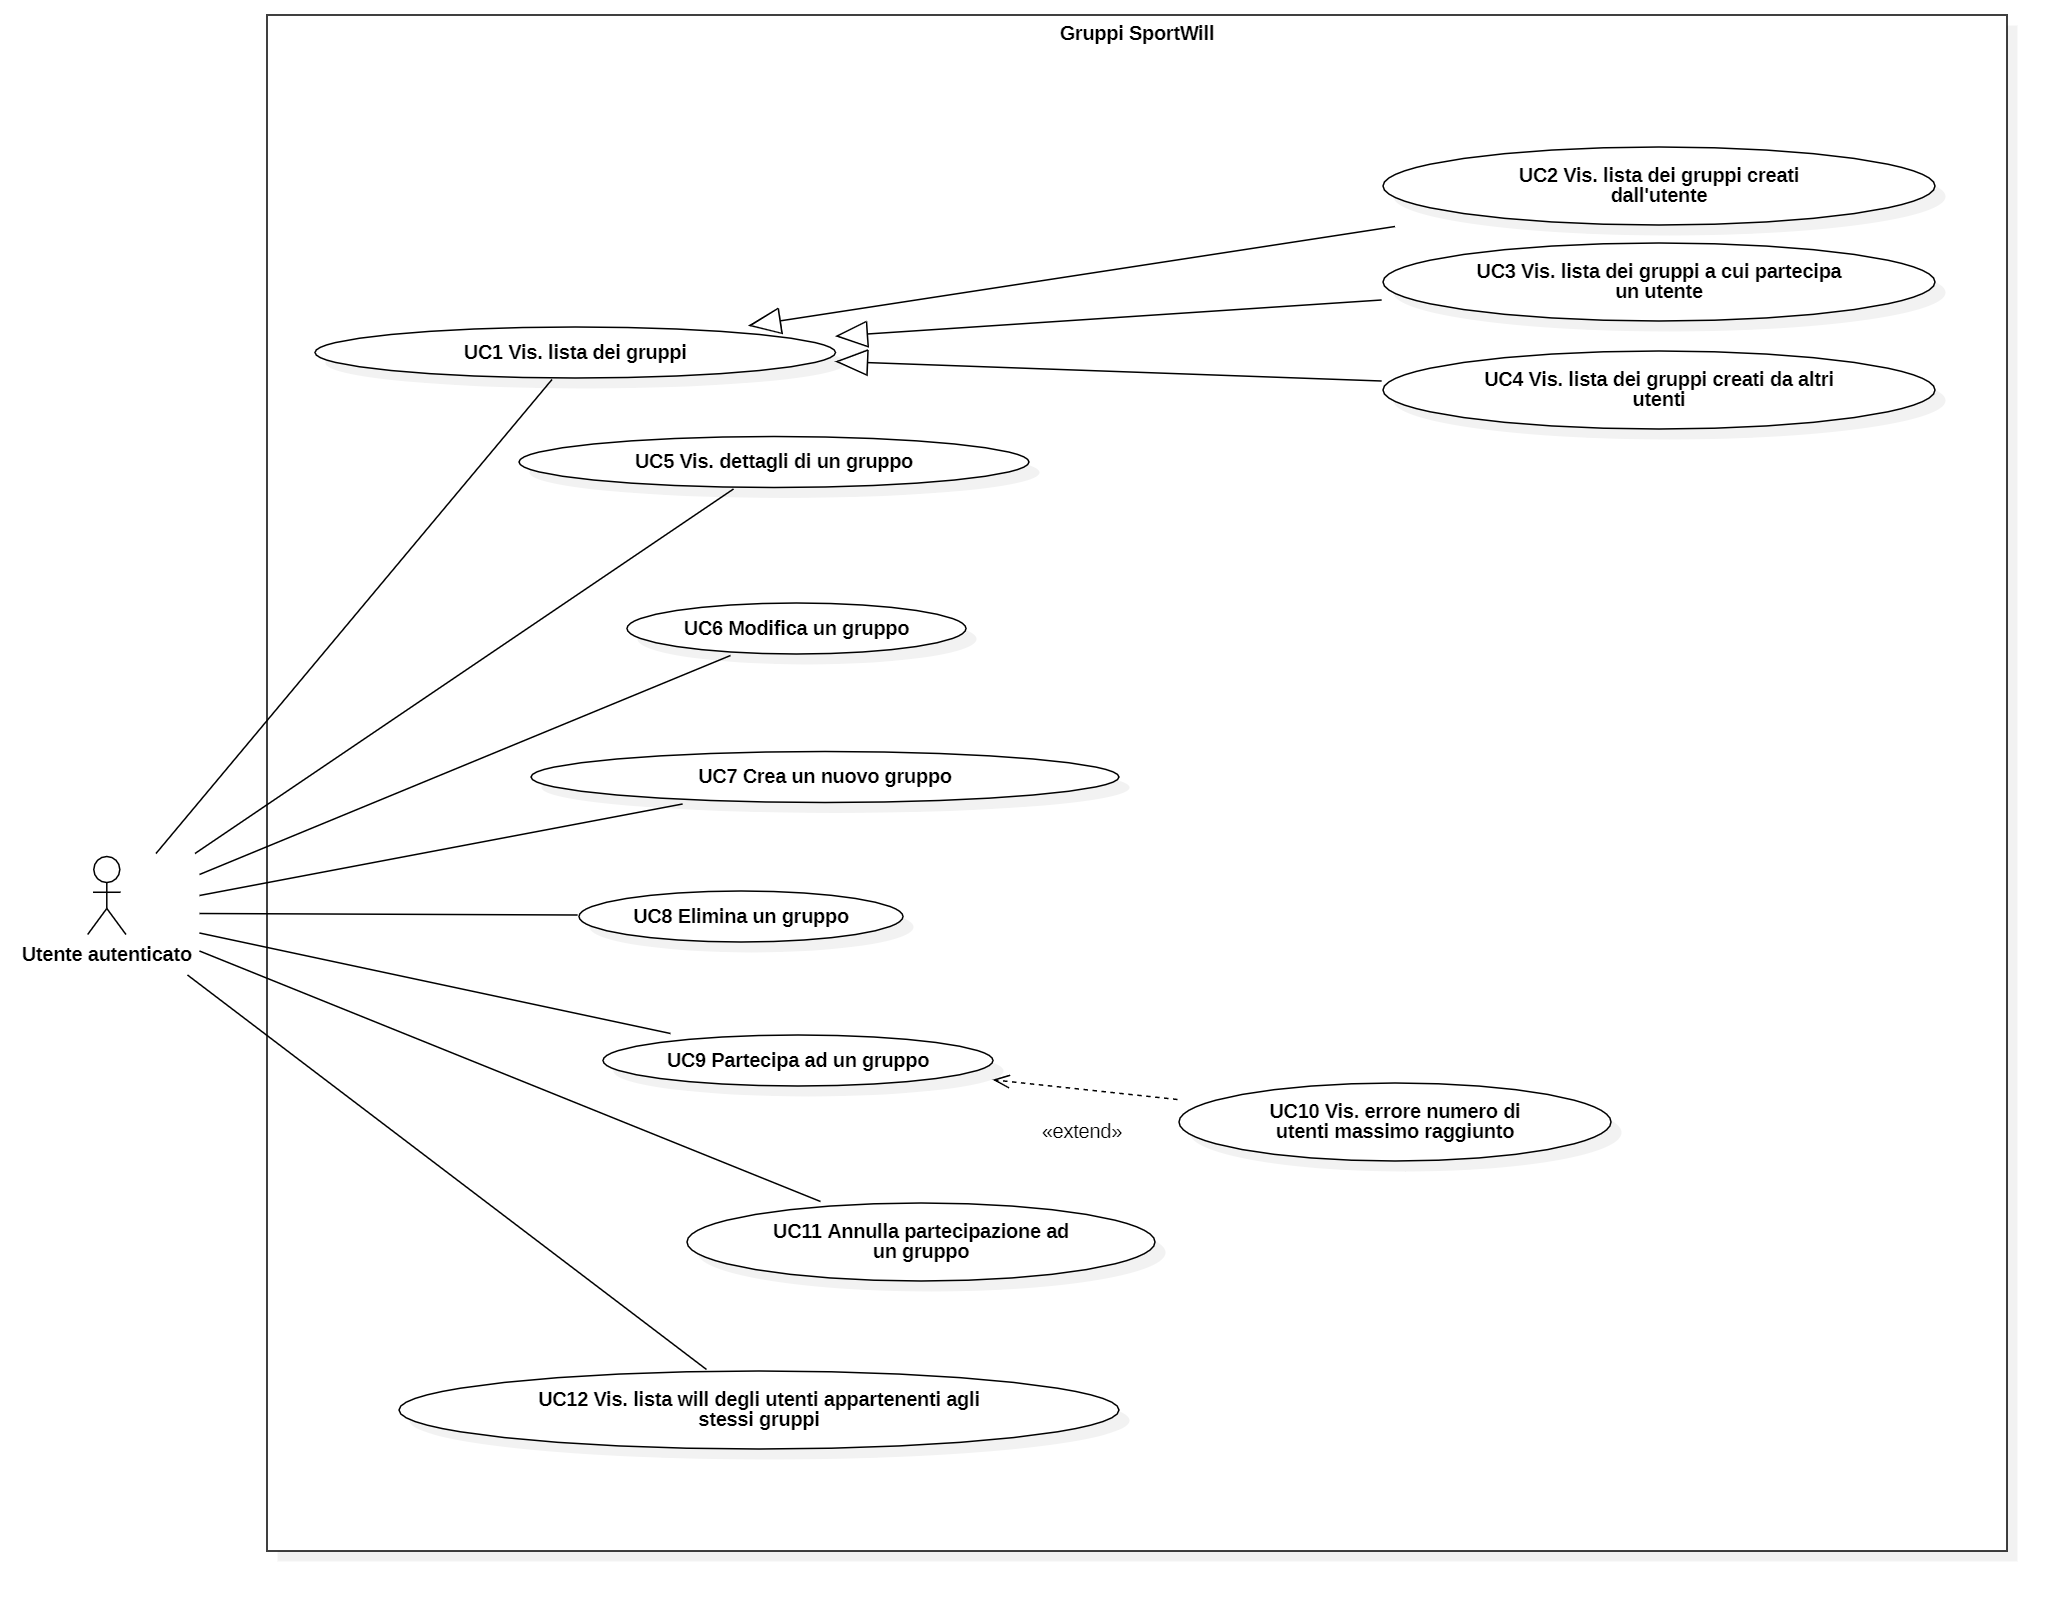
\includegraphics[width=1\columnwidth]{usecase/diagramma generale dei casi d'uso.png} 
    \caption{Diagramma generale dei casi d'uso}
\end{figure}

\begin{usecase}{Visualizzazione lista dei gruppi}
    \usecaseactors{Utente autenticato}
    \usecasepre{L'utente ha aperto la \textit{web-app} ed è autenticato}
    \usecasedesc{L'utente vuole visualizzare la lista dei gruppi}
    \usecasepost{L'utente ha visualizzato la lista dei gruppi}
    \usecasescenarioprincipale{
        \begin{enumerate}[nolistsep]
            \item L'utente visualizza la lista dei gruppi.
        \end{enumerate}
    }
    \label{uc:scenario-visualizzazione-lista-gruppi}
\end{usecase}
\newpage

\begin{figure}[H] 
    \centering 
    \includegraphics[width=1.2\columnwidth]{usecase/sottocasi UC1.png} 
    \caption{UC1: Vis. lista dei gruppi}
\end{figure}

\begin{subusecase}{Visualizzazione singolo gruppo in lista}
    \label{sub:visualizzazione-singolo-gruppo}
    \usecaseactors{Utente autenticato}
    \usecasepre{L'utente ha aperto la \textit{web-app}, è autenticato e sta visualizzando la lista dei gruppi}
    \usecasedesc{L'utente vuole visualizzare un singolo gruppo nella lista dei gruppi}
    \usecasepost{L'utente ha visualizzato un singolo gruppo nella lista dei gruppi}
    \usecasescenarioprincipale{
        \begin{enumerate}[nolistsep]
            \item L'utente visualizza un singolo gruppo nella lista dei gruppi.
        \end{enumerate}
    }
\end{subusecase}

\begin{figure}[H] 
    \centering 
    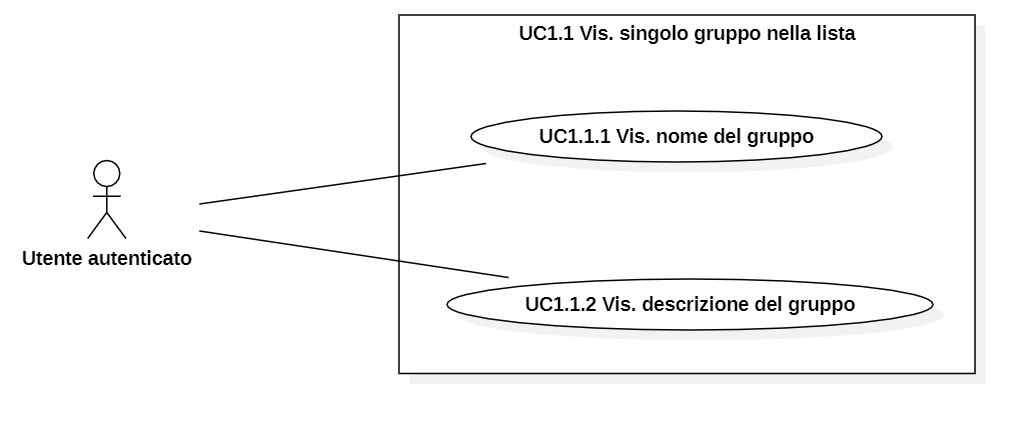
\includegraphics[width=1.2\columnwidth]{usecase/sottocasi UC1.1.png} 
    \caption{UC1.1: Vis. singolo gruppo in lista}
\end{figure}

\newpage

\begin{subsubusecase}{Visualizzazione nome del gruppo}
    \label{subsub:visualizzazione-nome-gruppo}
    \usecaseactors{Utente autenticato}
    \usecasepre{L'utente ha aperto la \textit{web-app}, è autenticato e sta visualizzando un gruppo dalla lista dei gruppi}
    \usecasedesc{L'utente vuole visualizzare il nome di un gruppo dalla lista dei gruppi}
    \usecasepost{L'utente ha visualizzato il nome di un gruppo dalla lista dei gruppi}
    \usecasescenarioprincipale{
        \begin{enumerate}[nolistsep]
            \item L'utente visualizza il nome di un gruppo dalla lista dei gruppi.
        \end{enumerate}
    }
\end{subsubusecase}


\begin{subsubusecase}{Visualizzazione descrizione del gruppo}
    \label{subsub:visualizzazione-descrizione-gruppo}
    \usecaseactors{Utente autenticato}
    \usecasepre{L'utente ha aperto la \textit{web-app}, è autenticato e sta visualizzando un gruppo dalla lista dei gruppi}
    \usecasedesc{L'utente vuole visualizzare la descrizione di gruppo della lista dei gruppi}
    \usecasepost{L'utente ha visualizzato la descrizione di un gruppo dalla lista dei gruppi}
    \usecasescenarioprincipale{
        \begin{enumerate}[nolistsep]
            \item L'utente visualizza la descrizione di un gruppo dalla lista dei gruppi.
        \end{enumerate}
    }
\end{subsubusecase}


\begin{usecase}{Visualizzazione lista dei gruppi creati dall'utente}
    \label{uc:scenario-visualizzazione-lista-gruppi-creati}
    \usecaseactors{Utente autenticato}
    \usecasepre{L'utente ha aperto la \textit{web-app} ed è autenticato}
    \usecasedesc{L'utente vuole visualizzare la lista dei gruppi creati da lui}
    \usecasepost{L'utente ha visualizzato la lista dei gruppi creati da lui}
    \usecasescenarioprincipale{
        \begin{enumerate}[nolistsep]
            \item L'utente visualizza la lista dei gruppi creati da lui.
        \end{enumerate}
    }
\end{usecase}

\begin{usecase}{Visualizzazione lista dei gruppi a cui partecipa un utente}
    \label{uc:scenario-visualizzazione-lista-gruppi-partecipa}
    \usecaseactors{Utente autenticato}
    \usecasepre{L'utente ha aperto la \textit{web-app} ed è autenticato}
    \usecasedesc{L'utente vuole visualizzare la lista dei gruppi a cui partecipa}
    \usecasepost{L'utente ha visualizzato la lista dei gruppi a cui partecipa}
    \usecasescenarioprincipale{
        \begin{enumerate}[nolistsep]
            \item L'utente visualizza la lista dei gruppi a cui partecipa.
        \end{enumerate}
    }
\end{usecase}


\begin{usecase}{Visualizzazione lista dei gruppi creati da altri utenti}
    \label{uc:scenario-visualizzazione-lista-gruppi-altri}
    \usecaseactors{Utente autenticato}
    \usecasepre{L'utente ha aperto la \textit{web-app} ed è autenticato}
    \usecasedesc{L'utente vuole visualizzare la lista dei gruppi creati da altri utenti}
    \usecasepost{L'utente ha visualizzato la lista dei gruppi creati da altri utenti}
    \usecasescenarioprincipale{
        \begin{enumerate}[nolistsep]
            \item L'utente visualizza la lista dei gruppi creati da altri utenti.
        \end{enumerate}
    }
\end{usecase}


\begin{usecase}{Visualizzazione dettagli di un gruppo}
    \label{uc:scenario-visualizzazione-dettaglio-gruppo}
    \usecaseactors{Utente autenticato}
    \usecasepre{L'utente ha aperto la \textit{web-app} ed è autenticato}
    \usecasedesc{L'utente vuole visualizzare i dettagli di un gruppo}
    \usecasepost{L'utente ha visualizzato i dettagli di un gruppo}
    \usecasescenarioprincipale{
        \begin{enumerate}[nolistsep]
            \item L'utente visualizza i dettagli di un gruppo.
        \end{enumerate}
    }
\end{usecase}
\begin{figure}[H] 
    \centering 
    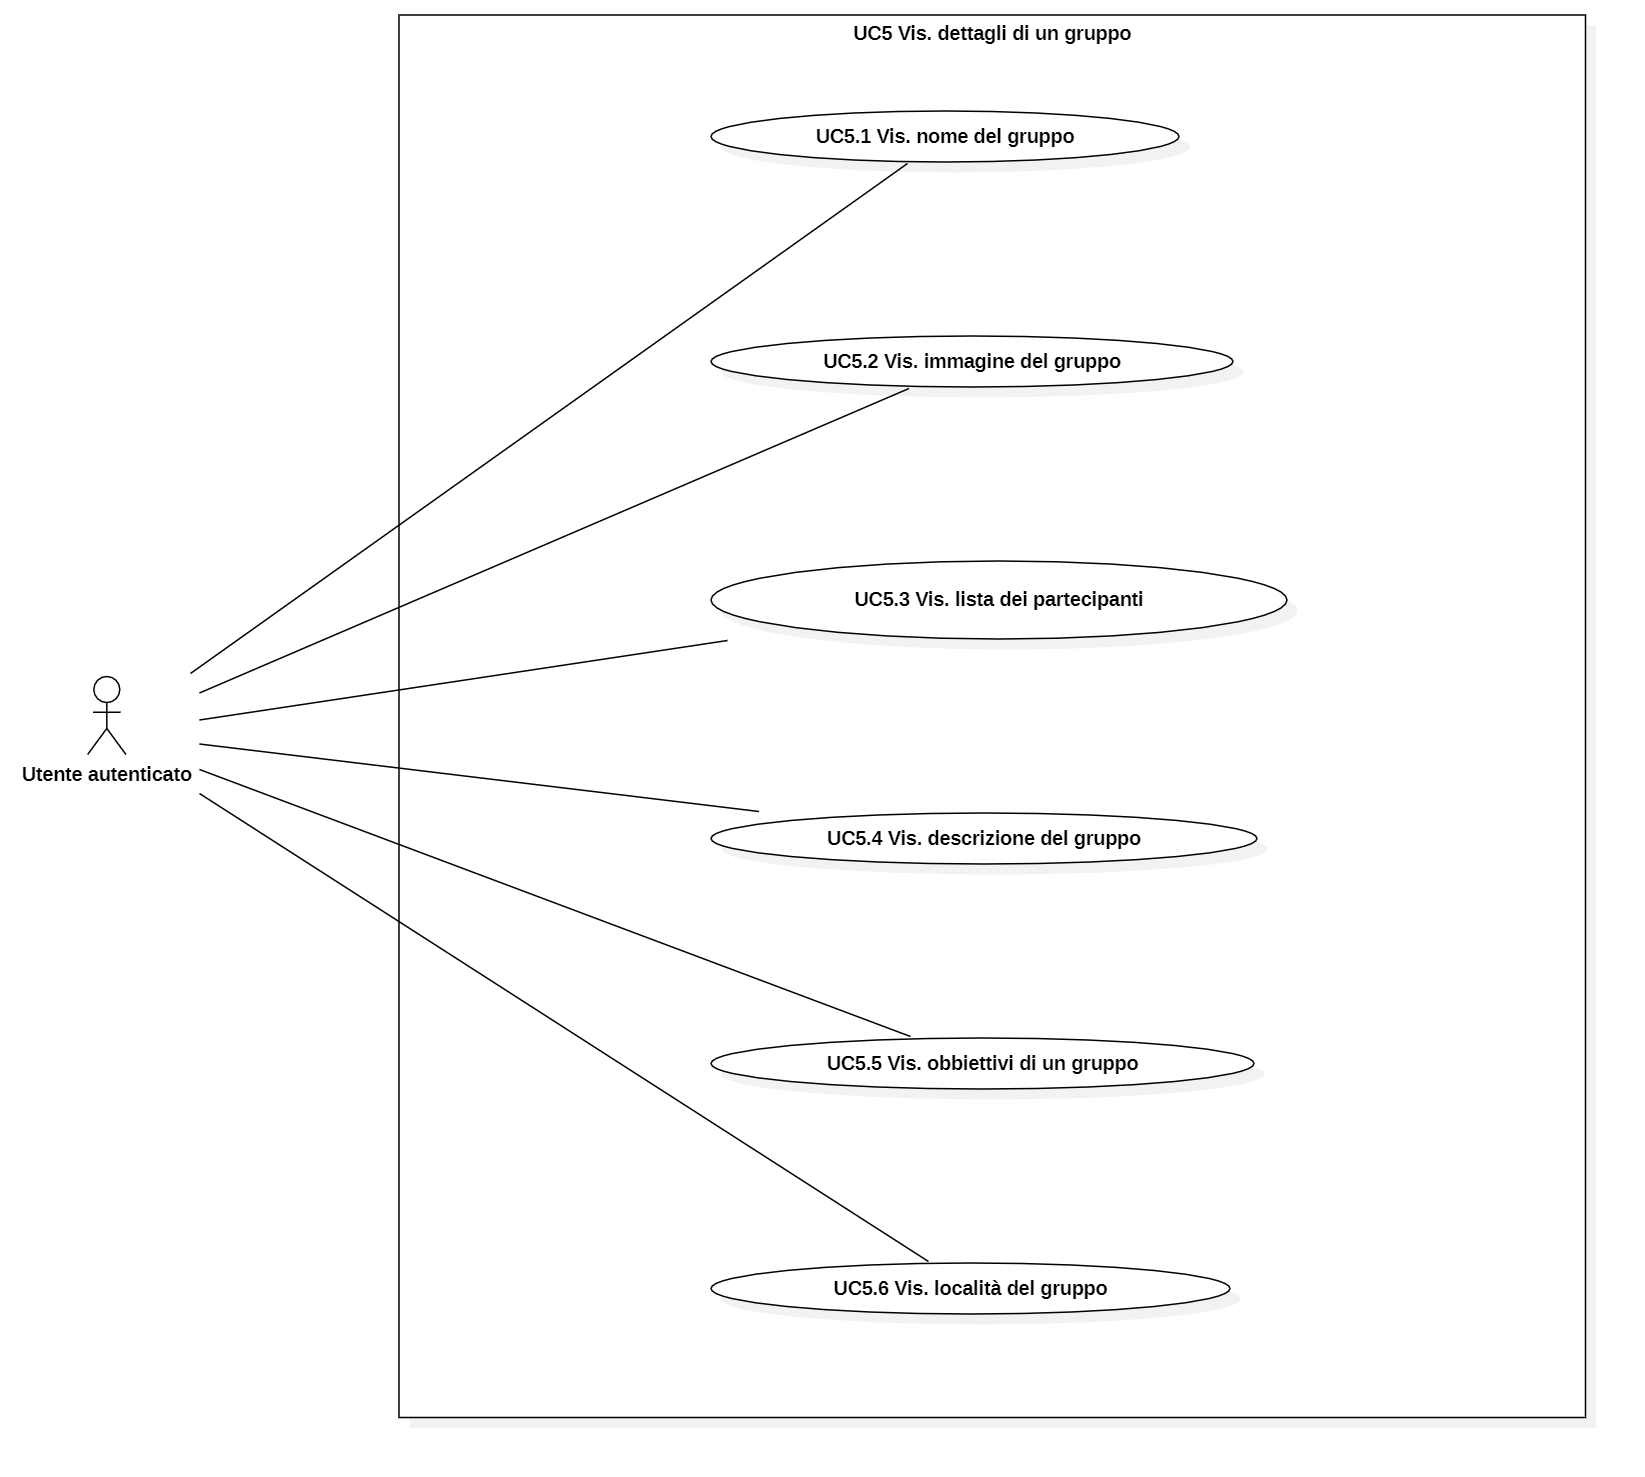
\includegraphics[width=1\columnwidth]{usecase/sottocasi UC5.png} 
    \caption{UC5: Vis. dettagli di un gruppo}
\end{figure}
\newpage


\begin{subusecase}{Visualizzazione nome del gruppo}
    \label{sub:visualizzazione-nome-gruppo}
    \usecaseactors{Utente autenticato}
    \usecasepre{L'utente ha aperto la \textit{web-app}, è autenticato e sta visualizzando i dettagli di un gruppo}
    \usecasedesc{L'utente vuole visualizzare il nome di un gruppo}
    \usecasepost{L'utente ha visualizzato il nome di un gruppo}
    \usecasescenarioprincipale{
        \begin{enumerate}[nolistsep]
            \item L'utente visualizza il nome di un gruppo.
        \end{enumerate}
    }
\end{subusecase}

\begin{subusecase}{Visualizzazione immagine del gruppo}
    \label{sub:visualizzazione-immagine-gruppo}
    \usecaseactors{Utente autenticato}
    \usecasepre{L'utente ha aperto la \textit{web-app}, è autenticato e sta visualizzando i dettagli di un gruppo}
    \usecasedesc{L'utente vuole visualizzare l'immagine di un gruppo}
    \usecasepost{L'utente ha visualizzato l'immagine di un gruppo}
    \usecasescenarioprincipale{
        \begin{enumerate}[nolistsep]
            \item L'utente visualizza l'immagine di un gruppo.
        \end{enumerate}
    }
\end{subusecase}

\begin{subusecase}{Visualizzazione lista dei partecipanti di un gruppo}
    \label{sub:visualizzazione-utenti-gruppo}
    \usecaseactors{Utente autenticato}
    \usecasepre{L'utente ha aperto la \textit{web-app}, è autenticato e sta visualizzando i dettagli di un gruppo}
    \usecasedesc{L'utente vuole visualizzare la lista dei partecipanti ad un gruppo}
    \usecasepost{L'utente ha visualizzato la lista dei partecipanti ad un gruppo}
    \usecasescenarioprincipale{
        \begin{enumerate}[nolistsep]
            \item L'utente visualizza la lista dei partecipanti ad un gruppo.
        \end{enumerate}
    }
\end{subusecase}

\begin{figure}[H] 
    \centering 
    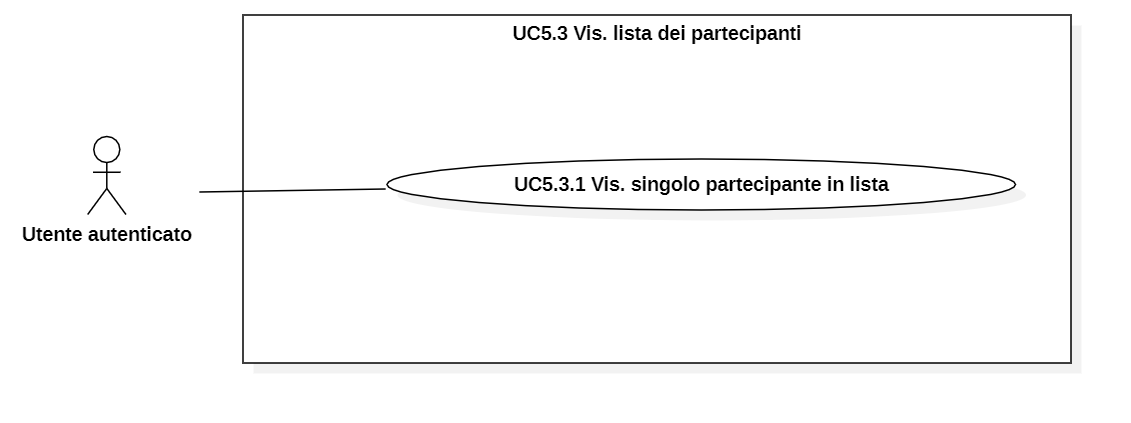
\includegraphics[width=1\columnwidth]{usecase/sottocasi UC5.3.png} 
    \caption{UC5.3: Vis. lista dei partecipanti di un gruppo}
\end{figure}

\begin{subsubusecase}{Visualizzazione singolo partecipante in lista}
    \label{subsub:visualizzazione-partecipanti-gruppo}
    \usecaseactors{Utente autenticato}
    \usecasepre{L'utente ha aperto la \textit{web-app}, è autenticato e sta visualizzando la lista dei partecipanti ad un gruppo}
    \usecasedesc{L'utente vuole visualizzare un partecipante dalla lista dei partecipanti ad un gruppo}
    \usecasepost{L'utente ha visualizzato un partecipante dalla lista dei partecipanti ad un gruppo}
    \usecasescenarioprincipale{
        \begin{enumerate}[nolistsep]
            \item L'utente visualizza un partecipante dalla lista dei partecipanti ad un gruppo.
        \end{enumerate}
    }
\end{subsubusecase}

\begin{figure}[H] 
    \centering 
    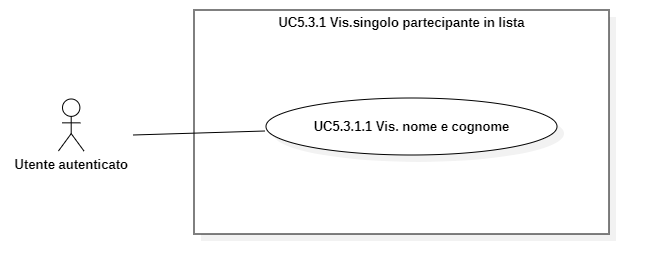
\includegraphics[width=1\columnwidth]{usecase/sottocasi UC5.3.1.png} 
    \caption{UC5.3.1: Vis. singolo partecipante in lista}
\end{figure}

\begin{subsubsubusecase}{Visualizzazione singolo partecipante in lista}
    \label{subsubsub:visualizzazione-singolo-partecipante-gruppo}
    \usecaseactors{Utente autenticato}
    \usecasepre{L'utente ha aperto la \textit{web-app}, è autenticato e sta visualizzando un partecipante dalla lista dei partecipanti}
    \usecasedesc{L'utente vuole visualizzare nome e cognome di un partecipante dalla lista dei partecipanti}
    \usecasepost{L'utente ha visualizzato nome e cognome di un partecipante dalla lista dei partecipanti}
    \usecasescenarioprincipale{
        \begin{enumerate}[nolistsep]
            \item L'utente ha visualizza nome e cognome di un partecipante dalla lista dei partecipanti.
        \end{enumerate}
    }
\end{subsubsubusecase}

\begin{subusecase}{Visualizzazione descrizione del gruppo}
    \label{sub:visualizzazione-descrizione-gruppo}
    \usecaseactors{Utente autenticato}
    \usecasepre{L'utente ha aperto la \textit{web-app}, è autenticato e sta visualizzando i dettagli di un gruppo}
    \usecasedesc{L'utente vuole visualizzare la descrizione di un gruppo}
    \usecasepost{L'utente ha visualizzato la descrizione di un gruppo}
    \usecasescenarioprincipale{
        \begin{enumerate}[nolistsep]
            \item L'utente visualizza la descrizione di un gruppo.
        \end{enumerate}
    }
\end{subusecase}

\begin{subusecase}{Visualizzazione obbiettivi del gruppo}
    \label{sub:visualizzazione-obbiettivi-gruppo}
    \usecaseactors{Utente autenticato}
    \usecasepre{L'utente ha aperto la \textit{web-app}, è autenticato e sta visualizzando i dettagli di un gruppo}
    \usecasedesc{L'utente vuole visualizzare gli obbiettivi di un gruppo}
    \usecasepost{L'utente ha visualizzato gli obbiettivi di un gruppo}
    \usecasescenarioprincipale{
        \begin{enumerate}[nolistsep]
            \item L'utente visualizza gli obbiettivi di un gruppo.
        \end{enumerate}
    }
\end{subusecase}


\begin{subusecase}{Visualizzazione località del gruppo}
    \label{sub:visualizzazione-località-gruppo}
    \usecaseactors{Utente autenticato}
    \usecasepre{L'utente ha aperto la \textit{web-app}, è autenticato e sta visualizzando i dettagli di un gruppo}
    \usecasedesc{L'utente vuole visualizzare la località di un gruppo}
    \usecasepost{L'utente ha visualizzato la località di un gruppo}
    \usecasescenarioprincipale{
        \begin{enumerate}[nolistsep]
            \item L'utente visualizza la località di un gruppo.
        \end{enumerate}
    }
\end{subusecase}

\begin{usecase}{Modifica di un gruppo}
    \label{uc:scenario-modifica-gruppo}
    \usecaseactors{Utente autenticato}
    \usecasepre{L'utente ha aperto la \textit{web-app} ed è autenticato}
    \usecasedesc{L'utente vuole modificare i dettagli di un gruppo}
    \usecasepost{L'utente ha modificato i dettagli di un gruppo}
    \usecasescenarioprincipale{
        \begin{enumerate}[nolistsep]
            \item L'utente modifica i dettagli di un gruppo.
        \end{enumerate}
    }
\end{usecase}

\newpage

\begin{figure}[H] 
    \centering 
    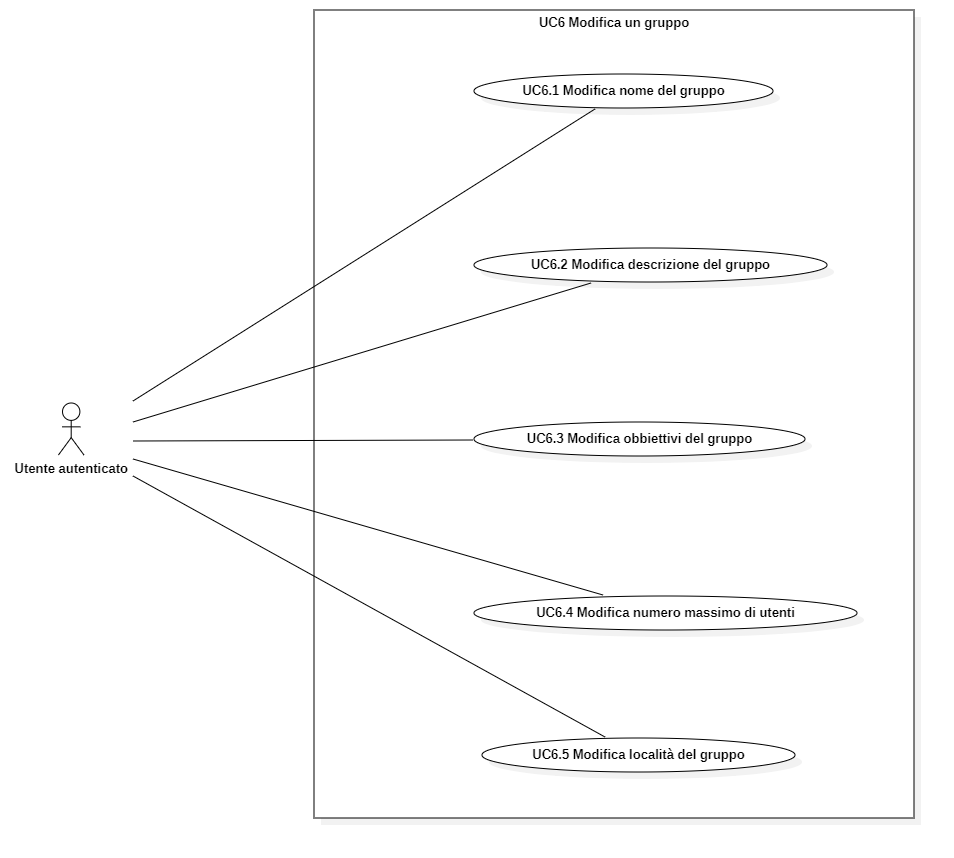
\includegraphics[scale=0.17]{usecase/sottocasi UC6.png} 
    \caption{UC6: Modifica di un gruppo}
\end{figure}

\begin{subusecase}{Modifica nome del gruppo}
    \label{sub:modifica-nome-gruppo}
    \usecaseactors{Utente autenticato}
    \usecasepre{L'utente ha aperto la \textit{web-app}, è autenticato e sta modificando i dettagli di un gruppo}
    \usecasedesc{L'utente vuole modificare il nome di un gruppo}
    \usecasepost{L'utente ha modificato il nome di un gruppo}
    \usecasescenarioprincipale{
        \begin{enumerate}[nolistsep]
            \item L'utente modifica il nome di un gruppo.
        \end{enumerate}
    }
\end{subusecase}

\begin{subusecase}{Modifica descrizione del gruppo}
    \label{sub:modifica-descrizione-gruppo}
    \usecaseactors{Utente autenticato}
    \usecasepre{L'utente ha aperto la \textit{web-app}, è autenticato e sta modificando i dettagli di un gruppo}
    \usecasedesc{L'utente vuole modificare la descrizione di un gruppo}
    \usecasepost{L'utente ha modificato la descrizione di un gruppo}
    \usecasescenarioprincipale{
        \begin{enumerate}[nolistsep]
            \item L'utente modifica la descrizione di un gruppo.
        \end{enumerate}
    }
\end{subusecase}

\begin{subusecase}{Modifica obbiettivi del gruppo}
    \label{sub:modifica-obbiettivi-gruppo}
    \usecaseactors{Utente autenticato}
    \usecasepre{L'utente ha aperto la \textit{web-app}, è autenticato e sta modificando i dettagli di un gruppo}
    \usecasedesc{L'utente vuole modificare gli obbiettivi di un gruppo}
    \usecasepost{L'utente ha modificato gli obbiettivi di un gruppo}
    \usecasescenarioprincipale{
        \begin{enumerate}[nolistsep]
            \item L'utente modifica gli obbiettivi di un gruppo.
        \end{enumerate}
    }
\end{subusecase}


\begin{subusecase}{Modifica numero massimo di utenti}
    \label{sub:modifica-numero-utenti-gruppo}
    \usecaseactors{Utente autenticato}
    \usecasepre{L'utente ha aperto la \textit{web-app}, è autenticato e sta modificando i dettagli di un gruppo}
    \usecasedesc{L'utente vuole modificare il numero massimo di utenti di un gruppo}
    \usecasepost{L'utente ha modificato il numero massimo di utenti di un gruppo}
    \usecasescenarioprincipale{
        \begin{enumerate}[nolistsep]
            \item L'utente modifica il numero massimo di utenti di un gruppo.
        \end{enumerate}
    }
\end{subusecase}

\begin{subusecase}{Modifica località del gruppo}
    \label{sub:modifica-località-gruppo}
    \usecaseactors{Utente autenticato}
    \usecasepre{L'utente ha aperto la \textit{web-app}, è autenticato e sta modificando i dettagli di un gruppo}
    \usecasedesc{L'utente vuole modificare la località di un gruppo}
    \usecasepost{L'utente ha modificato la località di un gruppo}
    \usecasescenarioprincipale{
        \begin{enumerate}[nolistsep]
            \item L'utente modifica la località di un gruppo.
        \end{enumerate}
    }
\end{subusecase}

\begin{subusecase}{Rimozione utente}
    \label{sub:-gruppo}
    \usecaseactors{Utente autenticato}
    \usecasepre{L'utente ha aperto la \textit{web-app}, è autenticato e sta modificando i dettagli di un gruppo}
    \usecasedesc{L'utente vuole rimuovere un utente dal gruppo}
    \usecasepost{L'utente ha rimosso un utente dal gruppo}
    \usecasescenarioprincipale{
        \begin{enumerate}[nolistsep]
            \item L'utente rimuove un utente dal gruppo.
        \end{enumerate}
    }
\end{subusecase}

\begin{usecase}{Crea un nuovo gruppo}
    \label{uc:scenario-creazione-nuovo-gruppo}
    \usecaseactors{Utente autenticato}
    \usecasepre{L'utente ha aperto la \textit{web-app} ed è autenticato}
    \usecasedesc{L'utente vuole creare un nuovo gruppo}
    \usecasepost{L'utente ha creato un nuovo gruppo}
    \usecasescenarioprincipale{
        \begin{enumerate}[nolistsep]
            \item L'utente crea un nuovo gruppo.
        \end{enumerate}
    }
\end{usecase}

\begin{figure}[H] 
    \centering 
    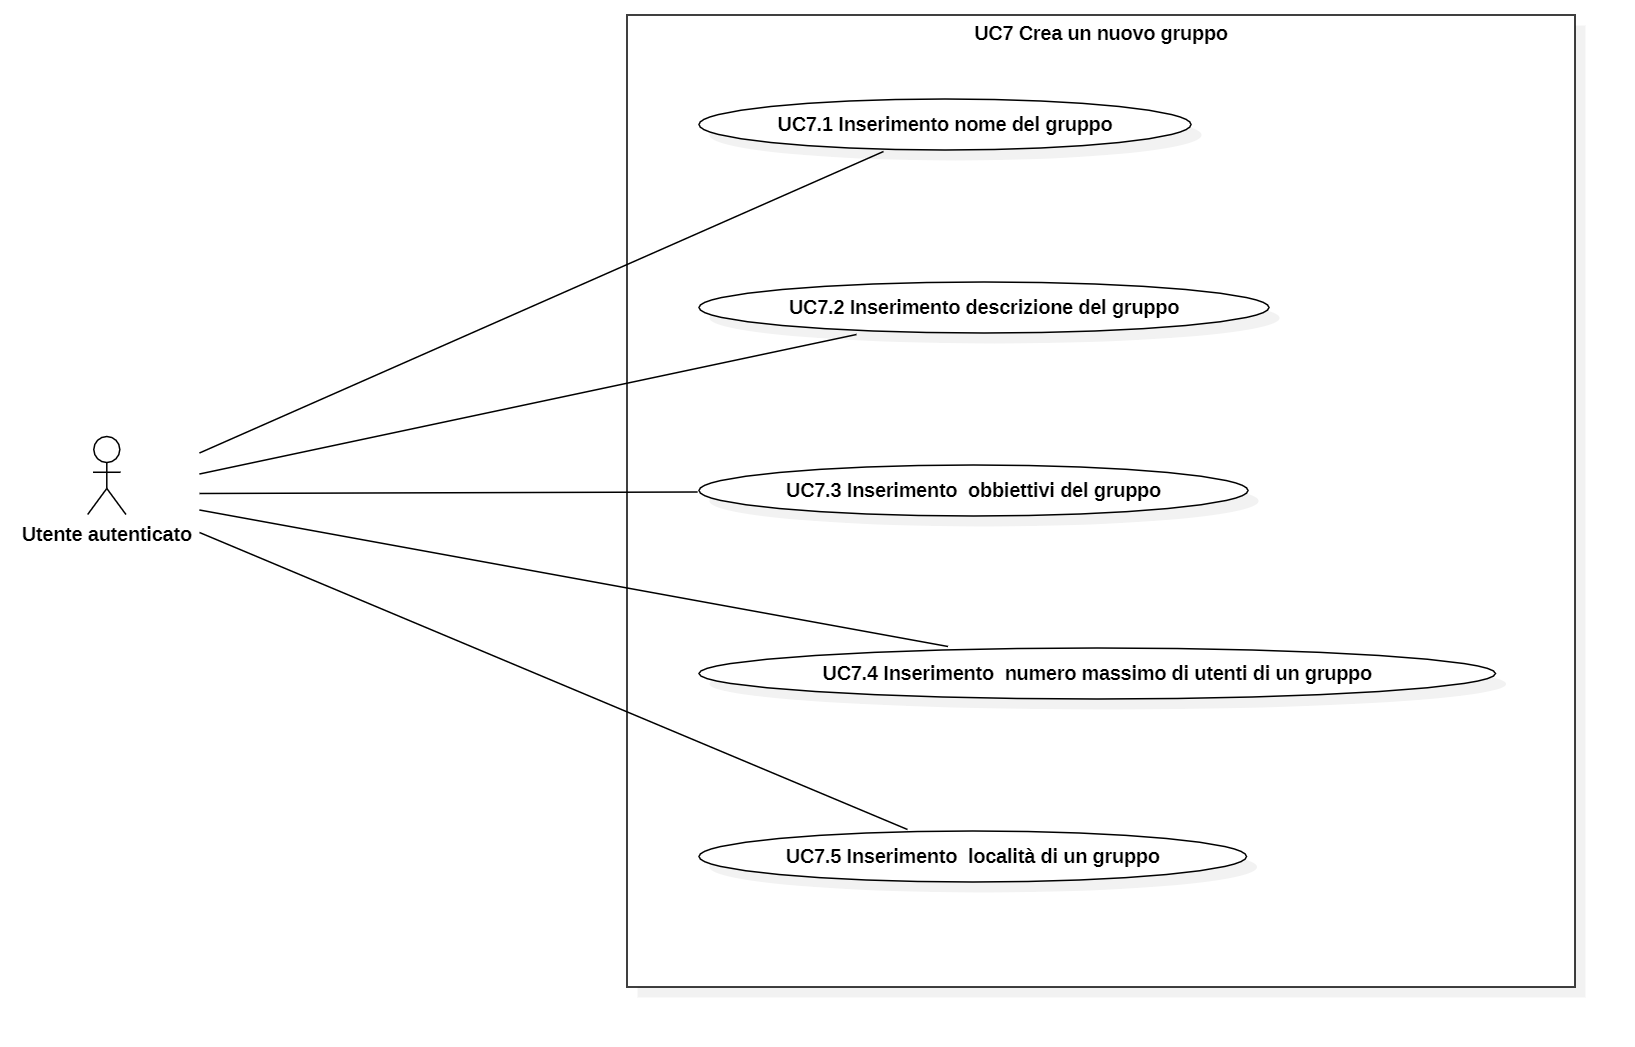
\includegraphics[width=1\columnwidth]{usecase/sottocasi UC7.png} 
    \caption{UC7: Crea un nuovo gruppo}
\end{figure}

\begin{subusecase}{Inserimento nome del gruppo}
    \label{sub:inserimento-nome-gruppo}
    \usecaseactors{Utente autenticato}
    \usecasepre{L'utente ha aperto la \textit{web-app}, è autenticato e sta creando un nuovo gruppo}
    \usecasedesc{L'utente vuole inserire il nome del gruppo}
    \usecasepost{L'utente ha inserito il nome del gruppo}
    \usecasescenarioprincipale{
        \begin{enumerate}[nolistsep]
            \item L'utente inserisce il nome del gruppo.
        \end{enumerate}
    }
\end{subusecase}


\begin{subusecase}{Inserimento descrizione del gruppo}
    \label{sub:inserimento-descrizione-gruppo}
    \usecaseactors{Utente autenticato}
    \usecasepre{L'utente ha aperto la \textit{web-app}, è autenticato e sta creando un nuovo gruppo}
    \usecasedesc{L'utente vuole inserire la descrizione del gruppo}
    \usecasepost{L'utente ha inserito la descrizione del gruppo}
    \usecasescenarioprincipale{
        \begin{enumerate}[nolistsep]
            \item L'utente inserisce la descrizione del gruppo.
        \end{enumerate}
    }
\end{subusecase}

\begin{subusecase}{Inserimento obbiettivi del gruppo}
    \label{sub:inserimento-obbiettivi-gruppo}
    \usecaseactors{Utente autenticato}
    \usecasepre{L'utente ha aperto la \textit{web-app}, è autenticato e sta creando un nuovo gruppo}
    \usecasedesc{L'utente vuole inserire gli obbiettivi del gruppo}
    \usecasepost{L'utente ha inserito gli obbiettivi del gruppo}
    \usecasescenarioprincipale{
        \begin{enumerate}[nolistsep]
            \item L'utente inserisce gli obbiettivi del gruppo.
        \end{enumerate}
    }
\end{subusecase}


\begin{subusecase}{Inserimento numero massimo di utenti nel gruppo}
    \label{sub:inserimento-numero-utenti-gruppo}
    \usecaseactors{Utente autenticato}
    \usecasepre{L'utente ha aperto la \textit{web-app}, è autenticato e sta creando un nuovo gruppo}
    \usecasedesc{L'utente vuole inserire il numero massimo di utenti del gruppo}
    \usecasepost{L'utente ha inserito il numero massimo di utenti del gruppo}
    \usecasescenarioprincipale{
        \begin{enumerate}[nolistsep]
            \item L'utente inserisce il numero massimo di utenti del gruppo.
        \end{enumerate}
    }
\end{subusecase}

\begin{subusecase}{Inserimento località del gruppo}
    \label{sub:inserimento-località-gruppo}
    \usecaseactors{Utente autenticato}
    \usecasepre{L'utente ha aperto la \textit{web-app}, è autenticato e sta creando un nuovo gruppo}
    \usecasedesc{L'utente vuole inserire la località del gruppo}
    \usecasepost{L'utente ha inserito la località del gruppo}
    \usecasescenarioprincipale{
        \begin{enumerate}[nolistsep]
            \item L'utente inserisce la località del gruppo.
        \end{enumerate}
    }
\end{subusecase}

\begin{usecase}{Elimina un gruppo}
    \label{uc:scenario-elimina-gruppo}
    \usecaseactors{Utente autenticato}
    \usecasepre{L'utente ha aperto la \textit{web-app} ed è autenticato}
    \usecasedesc{L'utente vuole eliminare un gruppo}
    \usecasepost{L'utente ha eliminato un gruppo}
    \usecasescenarioprincipale{
        \begin{enumerate}[nolistsep]
            \item L'utente elimina un gruppo.
        \end{enumerate}
    }
\end{usecase}


\begin{usecase}{Partecipa ad un gruppo}
    \label{uc:scenario-partecipa-gruppo}
    \usecaseactors{Utente autenticato}
    \usecasepre{L'utente ha aperto la \textit{web-app} ed è autenticato}
    \usecasedesc{L'utente vuole partecipare ad un gruppo}
    \usecasepost{L'utente ha partecipato ad un gruppo}
    \usecasescenarioprincipale{
        \begin{enumerate}[nolistsep]
            \item L'utente partecipa ad un gruppo.
        \end{enumerate}
    }
    \usecasealt{il gruppo ha raggiunto la capienza massima}
    \usecaseest{viene visualizzato un messaggio di errore a causa della capienza massima raggiunta dal gruppo}
\end{usecase}


\begin{usecase}{Visualizzazione errore numero di utenti massimo raggiunto}
    \label{uc:errore-numero-utenti}
    \usecaseactors{Utente autenticato}
    \usecasepre{L'utente ha aperto la \textit{web-app} ed è autenticato}
    \usecasedesc{L'utente vuole partecipare ad un gruppo}
    \usecasepost{L'utente non si unisce al gruppo}
    \usecasescenarioprincipale{
        \begin{enumerate}[nolistsep]
            \item l'utente sceglie di partecipare ad un gruppo;
            \item viene visualizzato un messaggio di errore a causa della capienza massima raggiunta dal gruppo.
        \end{enumerate}
    }
\end{usecase}


\begin{usecase}{Annulla partecipazione ad un gruppo}
    \label{uc:scenario-annulla-partecipazione}
    \usecaseactors{Utente autenticato}
    \usecasepre{L'utente ha aperto la \textit{web-app} ed è autenticato}
    \usecasedesc{L'utente vuole annullare la partecipazione ad un gruppo}
    \usecasepost{L'utente ha annullato la partecipazione ad un gruppo}
    \usecasescenarioprincipale{
        \begin{enumerate}[nolistsep]
            \item L'utente annulla la partecipazione ad un gruppo.
        \end{enumerate}
    }
\end{usecase}

\begin{usecase}{Visualizzazione lista delle will degli utenti appartenenti agli stessi gruppi}
    \label{uc:scenario-visualizzazione-will}
    \usecaseactors{Utente autenticato}
    \usecasepre{L'utente ha aperto la \textit{web-app} ed è autenticato}
    \usecasedesc{L'utente vuole visualizzare la lista delle will degli utenti appartenenti agli stessi gruppi}
    \usecasepost{L'utente ha visualizzato la lista delle will degli utenti appartenenti agli stessi gruppi}
    \usecasescenarioprincipale{
        \begin{enumerate}[nolistsep]
            \item L'utente visualizza la lista delle will degli utenti appartenenti agli stessi gruppi.
        \end{enumerate}
    }
\end{usecase}

\newpage 

\begin{figure}[H] 
    \centering 
    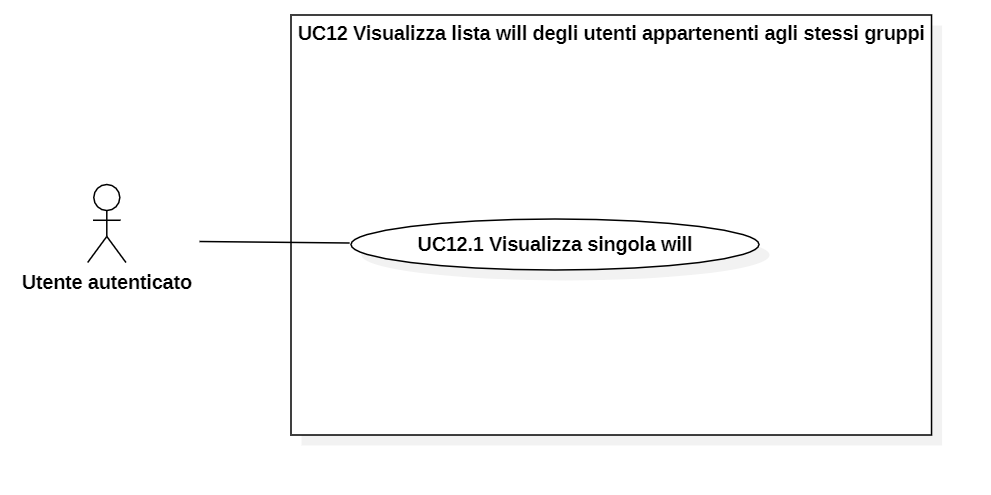
\includegraphics[width=1.2\columnwidth]{usecase/sottocasi UC12.png} 
    \caption{UC12: Vis. lista will degli utenti appartenenti agli stessi gruppi}
\end{figure}

\begin{subusecase}{Visualizzazione singola will in lista}
    \label{sub:visualizzazione-singola-will}
    \usecaseactors{Utente autenticato}
    \usecasepre{L'utente ha aperto la \textit{web-app}, è autenticato e sta visualizzando la lista dei gruppi}
    \usecasedesc{L'utente vuole visualizzare una singola \gls{will} dalla lista delle \gls{will}}
    \usecasepost{L'utente ha visualizzato una singola \gls{will} dalla lista delle \gls{will}}
    \usecasescenarioprincipale{
        \begin{enumerate}[nolistsep]
            \item L'utente visualizza una singola \gls{will} dalla lista delle \gls{will}.
        \end{enumerate}
    }
\end{subusecase}

\begin{figure}[H] 
    \centering 
    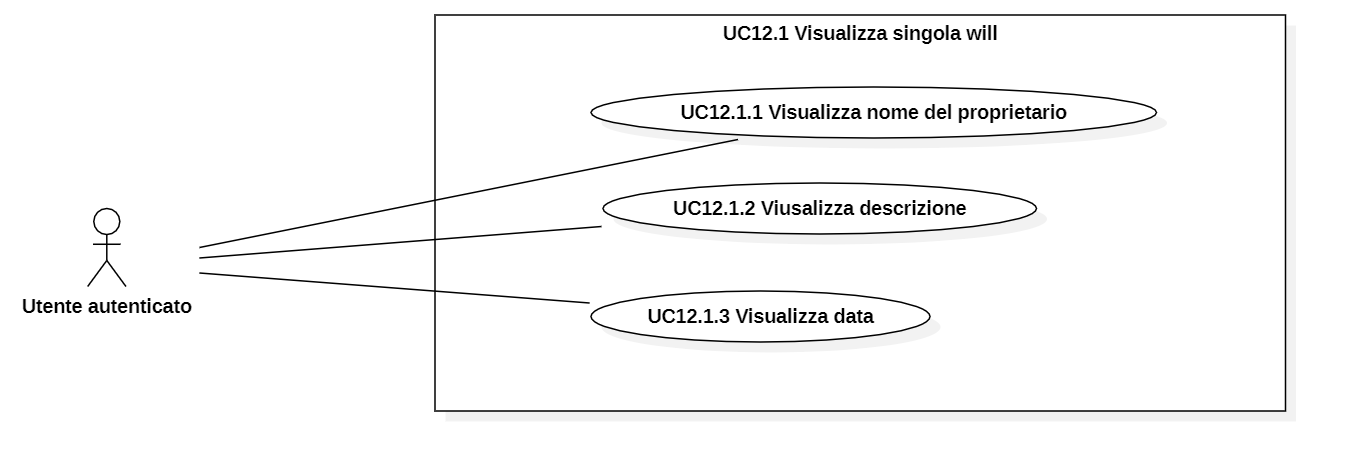
\includegraphics[width=1.2\columnwidth]{usecase/sottocasi UC12.1.png} 
    \caption{UC12.1: Vis. singola \textit{will}}
\end{figure}


\begin{subsubusecase}{Visualizzazione nome del proprietario}
    \label{subsub:visualizzazione-will-nome-proprietario}
    \usecaseactors{Utente autenticato}
    \usecasepre{L'utente ha aperto la \textit{web-app}, è autenticato e sta visualizzando un \gls{will} dalla lista delle \gls{will}}
    \usecasedesc{L'utente vuole visualizzare il nome del proprietario della \gls{will}}
    \usecasepost{L'utente ha visualizzato il nome del proprietario della \gls{will}}
    \usecasescenarioprincipale{
        \begin{enumerate}[nolistsep]
            \item L'utente visualizza il nome del proprietario della \gls{will}.
        \end{enumerate}
    }
\end{subsubusecase}

\begin{subsubusecase}{Visualizzazione descrizione}
    \label{subsub:visualizzazione-will-descrizione}
    \usecaseactors{Utente autenticato}
    \usecasepre{L'utente ha aperto la \textit{web-app}, è autenticato e sta visualizzando un \gls{will} dalla lista delle \gls{will}}
    \usecasedesc{L'utente vuole visualizzare la descrizione della \gls{will}}
    \usecasepost{L'utente ha visualizzato la descrizione della \gls{will}}
    \usecasescenarioprincipale{
        \begin{enumerate}[nolistsep]
            \item L'utente visualizza la descrizione della \gls{will}.
        \end{enumerate}
    }
\end{subsubusecase}

\begin{subsubusecase}{Visualizzazione data}
    \label{subsub:visualizzazione-will-data}
    \usecaseactors{Utente autenticato}
    \usecasepre{L'utente ha aperto la \textit{web-app}, è autenticato e sta visualizzando un \gls{will} dalla lista delle \gls{will}}
    \usecasedesc{L'utente vuole visualizzare la data in cui verrà effettuata l'uscita}
    \usecasepost{L'utente ha visualizzato la data in cui verrà effettuata l'uscita}
    \usecasescenarioprincipale{
        \begin{enumerate}[nolistsep]
            \item L'utente visualizza la data in cui verrà effettuata l'uscita.
        \end{enumerate}
    }
\end{subsubusecase}


\section{Tracciamento dei requisiti}
Da un'attenta analisi dei requisiti e degli use case effettuata sul progetto è stata stilata la tabella che traccia i requisiti in rapporto agli use case.\\
Sono stati individuati diversi tipi di requisiti e si è quindi fatto utilizzo di un codice identificativo per distinguerli.\\
Il codice dei requisiti è così strutturato R(F/Q/V)(N/D/O) dove:
\begin{enumerate}[nolistsep]
	\item[R =] requisito
    \item[F =] funzionale
    \item[Q =] qualitativo
    \item[V =] di vincolo
    \item[N =] obbligatorio (necessario)
    \item[D =] desiderabile
    \item[Z =] opzionale
\end{enumerate}
Nelle tabelle \ref{tab:requisiti-funzionali}, \ref{tab:requisiti-qualitativi} e \ref{tab:requisiti-vincolo} sono riassunti i requisiti e il loro tracciamento con gli use case delineati in fase di analisi.
\begin{table}[H]%
\caption{Tabella del tracciamento dei requisti funzionali}
\label{tab:requisiti-funzionali}
\begin{tabularx}{\textwidth}{lXl}
\hline\hline
\textbf{Requisito} & \textbf{Descrizione} & \textbf{Use Case}\\
\hline
RFN-1     & L'interfaccia permette di configurare il tipo di sonde del test & UC1 \\
\hline
\end{tabularx}
\end{table}%

\begin{table}[H]%
\caption{Tabella del tracciamento dei requisiti qualitativi}
\label{tab:requisiti-qualitativi}
\begin{tabularx}{\textwidth}{lXl}
\hline\hline
\textbf{Requisito} & \textbf{Descrizione} & \textbf{Use Case}\\
\hline
RQD-1    & Le prestazioni del simulatore hardware deve garantire la giusta esecuzione dei test e non la generazione di falsi negativi & - \\
\hline
\end{tabularx}
\end{table}%

\begin{table}[H]%
\caption{Tabella del tracciamento dei requisiti di vincolo}
\label{tab:requisiti-vincolo}
\begin{tabularx}{\textwidth}{lXl}
\hline\hline
\textbf{Requisito} & \textbf{Descrizione} & \textbf{Use Case}\\
\hline
RVO-1    & La libreria per l'esecuzione dei test automatici deve essere riutilizzabile & - \\
\hline
\end{tabularx}
\end{table}%             % Kick-Off
% !TEX encoding = UTF-8
% !TEX TS-program = pdflatex
% !TEX root = ../tesi.tex

%**************************************************************
\chapter{Progettazione e codifica}
\label{cap:progettazione-codifica}
%**************************************************************

\intro{Il seguente capitolo descrive gli strumenti e la progettazione con cui sono 
state implementate le integrazione con la \textit{web-app} \productName.}\\

%**************************************************************
\section{Tecnologie}
\label{sec:tecnologie-strumenti}

Di seguito viene data una panoramica delle tecnologie e strumenti utilizzati.

\subsection*{Java}
Java è un linguaggio di programmazione e una piattaforma di elaborazione 
rilasciato per la prima volta da Sun Microsystems nel 1995. Si è evoluto da umili
 origini per sostenere gran parte del mondo digitale di oggi, fornendo una
 piattaforma affidabile su cui sono costruiti molti servizi e applicazioni. 
 Anche i nuovi prodotti, innovativi nei servizi digitali progettati per il futuro,  
 continuano a fare affidamento su Java.
%TODO: aggiungere bibliografia, link: https://java.com/en/download/help/whatis_java.html
\subsection*{Spring}
Spring è un \textit{framework} open source per lo sviluppo di applicazioni su piattaforma Java.
A questo \textit{framework} sono associati tanti altri progetti, che hanno nomi composti come 
Spring Boot, Spring Data, Spring Batch, etc. Questi progetti sono stati ideati per
fornire funzionalità aggiuntive al \textit{framework}.
%TODO: aggiungere bibliografia, link: https://it.wikipedia.org/wiki/Spring_Framework

\subsection*{Typescript}
%**************************************************************
TypeScript è un linguaggio di programmazione sviluppato e gestito da Microsoft. 
È un \gls{superset} di JavaScript, che permette di aggiungere la tipizzazione 
statica opzionale al linguaggio. TypeScript è progettato per lo sviluppo di applicazioni 
di grandi dimensioni e per la \gls{transcompilazione} in JavaScript. Poiché TypeScript è un \gls{superset} di JavaScript, anche i programmi JavaScript esistenti sono validi programmi TypeScript.
%TODO: aggiungere bibliografia, link: https://en.wikipedia.org/wiki/TypeScript

\subsection*{Angular}
%**************************************************************
Angular è un \textit{framework} JavaScript per applicazioni \textit{web} dinamiche, utilizzato in particolare per la creazione di \gls{spa} e \textit{web-app}. Consente di utilizzare HTML come linguaggio template e di estenderne la sintassi per esprimere le componenti di un'applicazione in modo chiaro e succinto.
%TODO: aggiungere bibliografia, link: https://psicografici.com/angular-js/#:~:text=Angular%20%C3%A8%20un%20framework%20JavaScript,in%20modo%20chiaro%20e%20succinto.

\subsection*{Angular Material}
%**************************************************************
Angular Material è una libreria sviluppata da Google nel 2014 progettata per aiutare a sviluppare pagine \textit{web} in modo strutturato. \\
I suoi componenti aiutano a creare pagine \textit{web} e applicazioni \textit{web} attraenti, coerenti e funzionali.
%TODO: aggiungere bibliografia, link: https://psicografici.com/angular-js/#:~:text=Angular%20%C3%A8%20un%20framework%20JavaScript,in%20modo%20chiaro%20e%20succinto.

\subsection*{Node.js}
Node.js è una piattaforma di sviluppo open source per l'esecuzione di codice JavaScript lato \textit{server}. Node è utile per sviluppare applicazioni che richiedono una connessione permanente dal \textit{browser} al \textit{server} ed è spesso utilizzato per applicazioni in tempo reale come chat, feed di notizie e di notifiche.\\
Node.js è utilizzato da Angular per gestire le dipendenze, permettendo la dichiarazione di due insiemi di dipendenze: per gli sviluppatori e per far funzionare l'applicativo. In questo modo è possibile differenziare quali librerie si possono tralasciare in fase di \textit{deploy} dell'applicazione perché, ad esempio, necessarie solo per effettuare i test.
%TODO: aggiungere bibliografia, link: https://whatis.techtarget.com/definition/Nodejs#:~:text=James%20Denman-,Node.,feeds%20and%20web%20push%20notifications.

%**************************************************************
\section{Progettazione}
\label{sec:progettazione}

\subsection{Back end}
\subsubsection{Architettura Spring Boot}
Spring Boot è un modulo di Spring \textit{framework}. Viene utilizzato per creare applicazioni \textit{stand-alone} di livello produttivo con il minimo sforzo.\\
Spring Boot segue un'architettura a strati, in cui ogni livello comunica con gli strati vicini.\\
Ci sono quattro strati in Spring Boot sono i seguenti:
\begin{itemize}
    \item \textbf{\textit{Presentation layer}:} gestisce le richieste HTTP, trasforma il il parametro da formato JSON in classe e autentica la richiesta, per poi trasferirla al \textit{business layer};
    \item \textbf{\textit{Business Layer}:} gestisce tutta la \textit{business logic}. Consiste in classi di servizio e utilizza servizi forniti dagli strati di accesso ai dati;
    \item \textbf{\textit{Persistence Layer}:} contiene tutta la \textit{storage logic}, e trasformando gli oggetti provenienti dalla \textit{business logic} in righe del \textit{database};
    \item \textbf{\textit{Database Layer}:} in questo strato sono effettuate le operazioni \gls{CRUD}.
\end{itemize}
\begin{figure}[H] 
    \centering 
    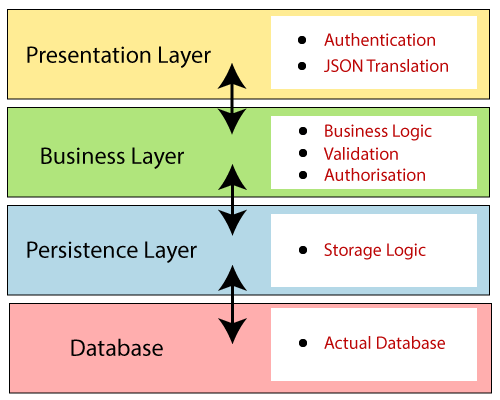
\includegraphics[scale=0.3]{spring-boot-architecture-layer.png} 
    \caption{Architettura a strati di Spring Boot}
\end{figure}

\subsubsection{Spring Boot Flow Architecture}
% https://codingjam.it/microservizi-in-java-con-spring-boot-e-spring-cloud/
\begin{figure}[H] 
    \centering 
    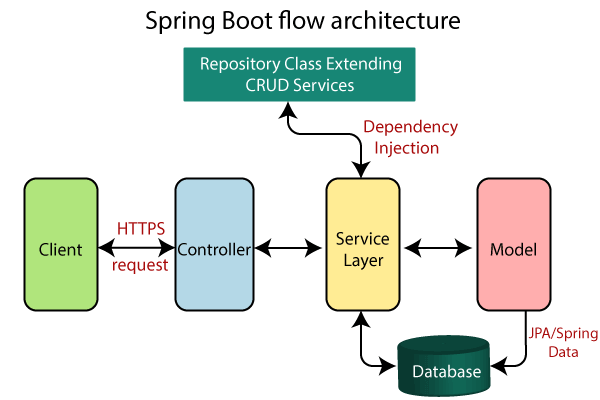
\includegraphics[width=1\columnwidth]{spring-boot-architecture.png} 
    \caption{Spring Boot \textit{workflow}}
\end{figure}
Il \textit{workflow} con cui vengono effettuate richieste HTTP utilizzando Spring Boot è il seguente:
\begin{itemize}
    \item il client esegue una richiesta HTTP (GET, POST, PUT O DELETE) ad un   \gls{endpoint} esposto;
    \item la richiesta va al \textit{controller}, che mappa la richiesta e la gestisce. Dopodiché chiama la \textit{service logic};
    \item nel \textit{service layer} viene eseguita la \textit{business logic}. Vengono eseguite le operazioni sulle classi mappate nel \textit{database};
    \item il \textit{repository} \textit{JpaRepository} esegue le operazioni sul database;
    \item una pagina \gls{JSP} viene restituita all'utente se non si è verificato un errore.
\end{itemize} 

\subsubsection{Organizzazione del codice}

\begin{figure}[H] 
    \centering 
    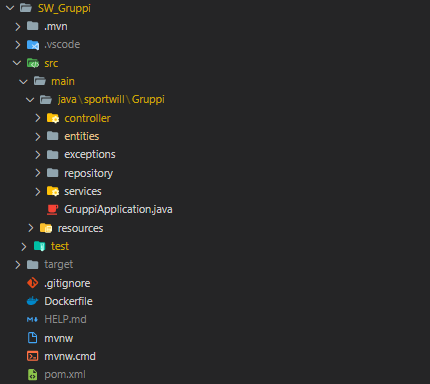
\includegraphics[width=0.65\columnwidth]{organizzazione_codice_spring.png} 
    \caption{Organizzazione del codice}
\end{figure}
Per inizializzare un nuovo \gls{microservizio} viene utilizzata l'estensione \textbf{Spring Initializr} per Visual Studio Code, che permette la generazione di un progetto per Spring Boot.\\
La cartella che contiene il codice del \gls{microservizio} è \texttt{src\textbackslash main\textbackslash java\textbackslash sportwill\textbackslash Gruppi}, che contiene le seguenti cartelle: 
\begin{itemize}
    \item \texttt{controller}: contiene la classe che mappa le richieste HTTP ai metodi specifici;
    \item \texttt{entities}: contiene le classi entità, ovvero classi che rappresentano delle tabelle in un \textit{database} relazionale e ogni istanza di entità corrisponde a una riga in quella tabella;
    \item \texttt{exceptions}: insieme di classi che estendono la classe Exception;
    \item \texttt{services}: classi che compongono il \textit{service layer}.


\end{itemize}
% TODO aggiungere alla bibliografia: https://microservices.io/patterns/apigateway.html
\subsubsection{Progettazione delle API}
Il \textit{back end} del progetto è strutturato a \glspl{microservizio}, ognuno contenente una business logic atta a soddisfare un certo tipo di richieste.\\
Il \textit{front end} comunica con il \textit{back end} attraverso gli \gls{endpoint} che ogni \gls{microservizio} espone. \\
Tuttavia, effettuare connessioni dirette fra \textit{front end} e ogni \gls{microservizio} presenta alcuni problemi, come: 
\begin{itemize}
    \item numerose connessioni a seconda della quantità dei \glspl{microservizio};
    \item i \glspl{microservizio} devono esporre pubblicamente il proprio \gls{IP}, causando problemi sia di sicurezza, dovuta all'esposizione degli indirizzi IP al mondo esterno, sia in fase di latenza, ovvero il tempo che intercorre tra l'invio di una richiesta ed una risposta tenderà ad essere
    sempre più alto.
\end{itemize}

\noindent Per far fronte a queste problematiche si è deciso di utilizzare un \gls{API Gateway}.\\
In questo modo, solamente un \gls{IP} sarà visibile pubblicamente, mentre quelli dei \glspl{microservizio} possono diventare privati.\\
Per quanto riguarda la latenza il \textit{front end} comunicherà attraverso l'\gls{API Gateway}, stabilendo solo le connessioni per la richiesta e la risposta, lasciando all'\gls{API Gateway} il compito di smistare le richieste al giusto \gls{microservizio}, permettendo una connessione più rapida rispetto  all'utilizzo di connessioni diverse per ogni \gls{microservizio}, essendo tutti all'interno dello stesso \textit{network}.

\subsection{Front end}
\subsubsection{Architettura Angular}
% TODO aggiungere alla bibliografia: https://angular.io/guide/architecture
Il componente principale di Angular è il \textbf{modulo}. Un modulo è un contenitore di funzionalità che sono es
poste ad altri moduli. Questa suddivisione in moduli rende la struttura dell'applicazione ordinata e il codice mantenibile.\\
Un elemento fondamentale di Angular è il \textbf{component}, ovvero delle classi che gestiscono le \textit{view} dell'applicazione e la loro logica.\\
I dati da visualizzare nella \textit{view} vengono forniti dalle classi dette \textbf{servizi}. Queste classi svolgono diverse funzioni, come per esempio  l'esecuzione delle richieste HTTP.\\  
Ad ogni component è associato un \textit{template}, ovvero del codice HTML in cui si definisce come viene visualizzato il component.\\
È possibile personalizzare il codice HTML utilizzando le \textbf{direttive}, ovvero delle classi che aggiungono un comportamento aggiuntivo agli elementi nelle applicazioni Angular. Le direttive integrate di Angular permettono di gestire moduli, elenchi, stili e ciò che gli utenti vedono.\\
È possibile creare un component che rappresenta la pagina completa, in cui inserire diversi component per ogni elemento contenuto in quella pagina.
Ogni component contenuto si occuperà così di gestire la grafica di quella determinata funzionalità e di comunicare con i servizi di cui necessita; sarà poi il component \enquote*{padre} a gestire la disposizione dei component utilizzati. 
\subsubsection{Organizzazione del codice}
% TODO: aggiungere questa sezione alla parte di codifica
\subsubsection{Progettazione delle maschere}
Con il \textit{tutor} aziendale è stato discusso come dovrebbe essere la grafica delle nuove maschere da aggiungere a \productName. Da queste discussioni è stato poi utilizzato \nameref{sub: Figma} per fare il \textit{mockup}, in modo da  testare come i vari elementi visivi lavorano insieme.\\
Durante la progettazione del \textit{mockup} è stato seguito lo stile presente nella \textit{web-app}, in modo da non disorientare l'utente durante la navigazione. \\
I risultati della progettazione sono riportati in seguito.
\begin{figure}[H] 
    \centering 
    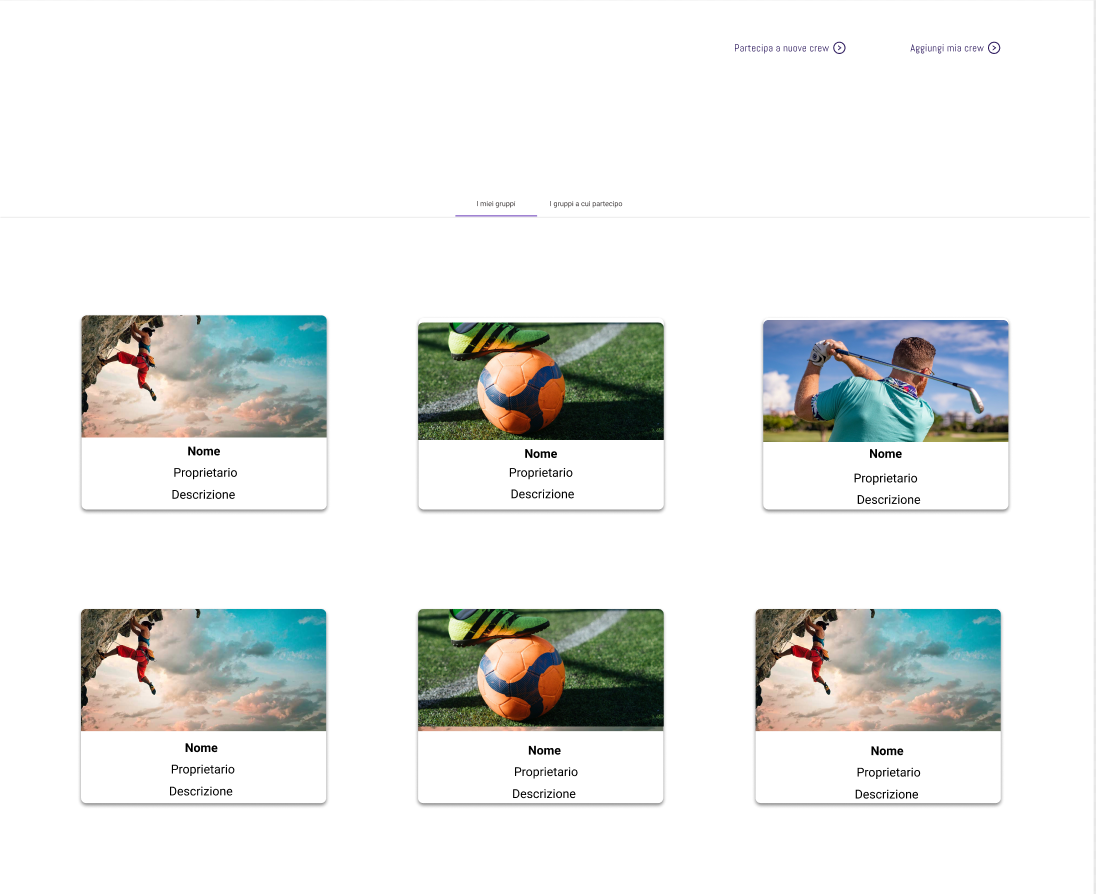
\includegraphics[scale=0.6]{mockup/le-mie-crew.png} 
    \caption{Mockup pagina per la visualizzazione dei gruppi creati dall'utente}
\end{figure}

\begin{figure}[H] 
    \centering 
    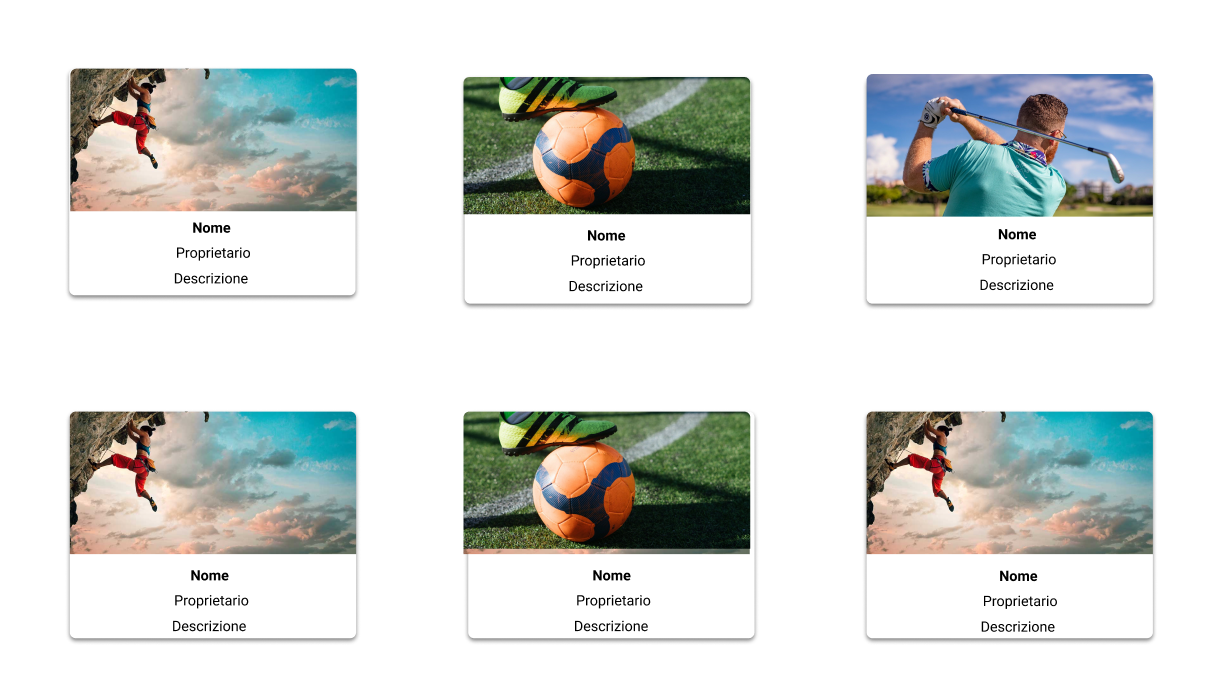
\includegraphics[scale=0.6]{mockup/lista-crew.png} 
    \caption{Mockup pagina per la visualizzazione dei gruppi a cui partecipa l'utente}
\end{figure}

\begin{figure}[H] 
    \centering 
    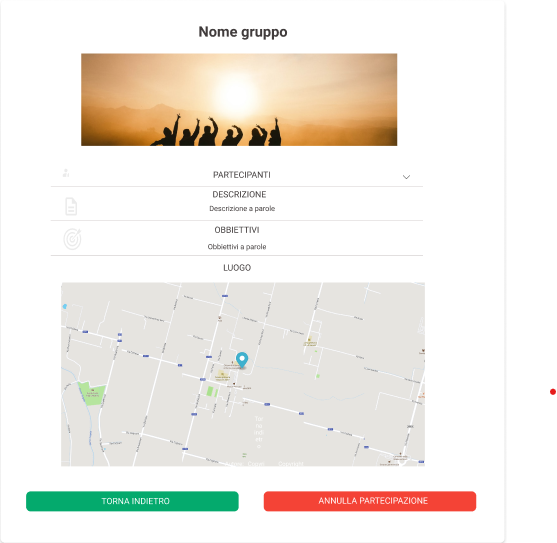
\includegraphics[scale=0.56]{mockup/dettagli-crew.png} 
    \caption{Mockup pagina per la visualizzazione dei dettagli di un gruppo}
\end{figure}

\begin{figure}[H] 
    \centering 
    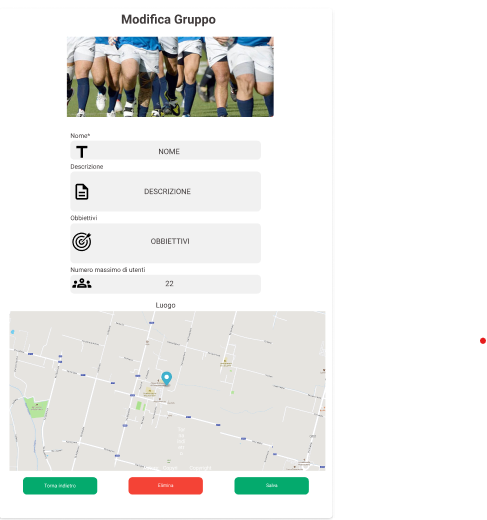
\includegraphics[scale=0.56]{mockup/modifica-crew.png} 
    \caption{Mockup pagina per la modifica dei dettagli di un gruppo}
\end{figure}

Come si può notare dalle immagini, sono stati omessi dalla progettazione l'header e il footer, in quanto sono già presenti nella \textit{web-app}.


% \subsubsection{Namespace 1} %**************************
% Descrizione namespace 1.

% \begin{namespacedesc}
%     \classdesc{Classe 1}{Descrizione classe 1}
%     \classdesc{Classe 2}{Descrizione classe 2}
% \end{namespacedesc}


%**************************************************************
\section{Design Pattern utilizzati}
\subsection{Microservizi}
% TODO: aggiungere alla bibliografia: https://aws.amazon.com/it/microservices/
I \glspl{microservizio} sono un approccio per sviluppare e organizzare l'architettura dei \textit{software} secondo cui quest'ultimi sono composti di servizi indipendenti di piccole dimensioni che comunicano tra loro tramite \gls{API} ben definite.\\
Nel contesto di questo progetto, sono stati implementati tre \glspl{microservizio}: 
\begin{itemize}
    \item \textbf{SW\_Gruppi}: \gls{microservizio} responsabile per la gestione delle funzionalità legate ai gruppi;
    \item \textbf{ApiGateway}: \gls{microservizio} che implementa il \textit{pattern} \nameref{sub: ApiGateway};
    \item \textbf{EurekaServer}: \gls{microservizio} che implementa il pattern \nameref{sub: ServiceRegistry}. 
\end{itemize}
\subsection{API Gateway}
\label{sub: ApiGateway}
Un \gls{API Gateway} è uno strumento di gestione delle \gls{API} che si situa tra un client e una raccolta di servizi \textit{back end}. Un \gls{API Gateway} si comporta come un proxy inverso per accettare tutte le chiamate \gls{API}, aggregare i vari servizi richiesti per gestirle e restituire i risultati appropriati.\\
Utilizzare un \gls{API Gateway} è vantaggioso perché: 
\begin{itemize}
    \item permette di centralizzare il punto di ingresso per le chiamate;
    \item permette di monitorare le risorse utilizzate;
    \item permette di proteggere un servizio che è aperto a tutti;
    \item latenza minore rispetto alla chiamata a diversi 
\end{itemize}
\subsection{Client-Side Service Discovery e Service Registry}
\begin{figure}[H] 
    \centering 
    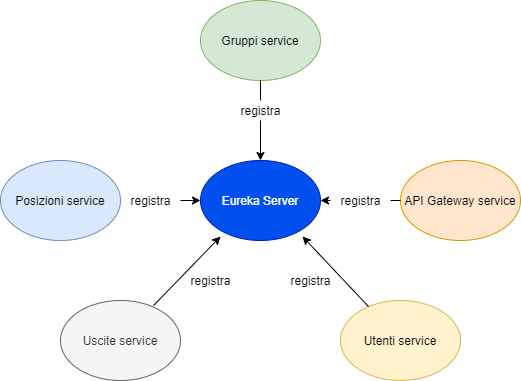
\includegraphics[scale=0.3]{progettazione/registrazione-servizi.png} 
    \caption{Diagramma concettuale che descrive la registrazione dei microservizi all'Eureka Server}
\end{figure}
%TODO: aggungere bibliografia: https://lalverma.medium.com/spring-boot-microservices-implementing-service-discovery-cfc98e49b74f, https://microservices.io/patterns/service-registry.html
I \glspl{microservizio} hanno una natura dinamica, in quanto è possibile che più istanze di un singolo \gls{microservizio} coesistano, probabilmente esponendo le loro \gls{API} in un indirizzo \gls{IP} diverso o una porta diversa. Queste evenienze portano all'impossibilità di: 
\begin{itemize}
    \item conoscere la posizione di qualsiasi istanza dei \glspl{microservizio};
    \item tenere traccia di tutte le istanze;
    \item selezionare un'istanza di \gls{microservizio}.
\end{itemize}
La soluzione a questi problemi è l'utilizzo del \textit{pattern} \textbf{\textit{Client-side Service Discovery}}, che fornisce un meccanismo che tiene traccia di tutti i servizi e delle relative istanze. Tutti i \glspl{microservizio} si registrano e continuano ad aggiornare regolarmente le proprie informazioni di rete.\\
Per registrare un \gls{microservizio} è stato utilizzato il \textit{pattern} 
\textbf{\textit{Service registry}}, applicato mediante un l'implementazione di un \textbf{Eureka Server}. L'Eureka Server è un \textit{database} di servizi che tiene traccia di ogni \gls{microservizio}, delle loro istanze e delle loro locazioni. I \glspl{microservizio} si registrano all'avvio dell'applicazione e vengono rimossi alla chiusura.\\
L'utilizzo di questi \textit{pattern}  permette ai servizi di comunicare fra di loro, ottenendo le informazioni degli altri servizi direttamente dall'Eureka Server.
\subsection{Dependency Injection}
\subsection{Singleton}
\subsection{Feature Service}
\subsection{Decorator}
\subsection{Lazy Loading}
\subsection{Observer}

%**************************************************************
\section{Codifica}
\subsection{Back end}

\subsubsection{Gruppi service}
\subsubsection{Modifica dei servizi esistenti}
\subsubsection{Api Gateway ed Eureka Server}
\subsubsection{Docker}

\subsection{Front end}
\subsubsection{Maschere}
\subsubsection{Componenti}             % Concept Preview
% !TEX encoding = UTF-8
% !TEX TS-program = pdflatex
% !TEX root = ../tesi.tex

%**************************************************************
\chapter{Verifica e validazione}
\label{cap:verifica-validazione}
%**************************************************************

\section{Accessibilità}
\subsection{Elementi di accessibilità}
Per rendere la navigazione al sito accessibile da tutte le categorie di utenti
sono stati fatti alcuni accorgimenti:
\begin{itemize}
    \item sono presenti gli attributi \textit{accesskey} con chiave uguale alla
          prima lettera della parola del \textit{tag label} associato, in modo da
          migliorare l'accessibilità alle \textit{form} da tastiera senza l'uso del
          \textit{mouse};
    \item tutte le immagini contengono i \textit{tag alt}, che sono stati
          lasciati vuoti nel caso servissero solo per il \textit{layout};
    \item è presente una barra di navigazione che aiuta a navigare nel sito;
    \item i \textit{form} contengono dei \textit{tag label} per ogni
          \textit{input}, tuttavia non sono stati aggiunti \textit{tag optgroup} o
          \textit{fieldset} in quanto sono utili nel caso di \textit{form} molto grandi,
          ma essendo presenti solo \textit{form} di piccole dimensioni è stato ritenuto
          non necessario;
    \item sono presenti degli aiuti contestuali che mostrano gli errori nel
          caso fossero presenti;
    \item è presente del testo nascosto utile agli utenti con disabilità
          visive, come il \textit{link} con la funzione  di saltare al contenuto, ovvero
          di permettere di non far leggere allo \gls{screen reader} la barra di
          navigazione, passando direttamente al contenuto, ed è presente all'inizio della
          navigazione per segnalare che le scorciatoie da tastiera sono attive;
    \item sono stati evitati testi scorrevoli, lampeggianti, barrati ed in
          generale \textit{font} troppo elaborati per agevolare la lettura.
\end{itemize}

\section{Verifica del GruppiService}
In parallelo con la fase di codifica del \gls{microservizio}
\nameref{par:GruppiService} è stata verificata la correttezza delle funzioni
presenti nella classe \texttt{GruppiController}. \\
Sono stati effettuati dei test di unità utilizzando \textbf{JUnit} e
\textbf{Mockito}, \gls{framework} di \textit{testing} per il linguaggio Java.\\
Per avere una reportistica dei test effettuati è stato utilizzato
\textbf{JaCoCo}, strumento che fornisce informazioni sulla \textit{lines
    coverage}, \textit{branches coverage} e \textit{cyclomatic complexity}.
L'attività di verifica si è rivelata molto proficua, permettendomi di agevolare
lo sviluppo in modo significativo, tanto da produrre un
grande quantitativo di test, con un elevata copertura di casistiche, garantendo
così qualità del prodotto.\\
Come dimostra la \textit{code coverage} (figura \ref{img:code-coverage}) è
stata raggiunta la massima copertura del codice, senza che questo inficiasse
sulle tempistiche programmate.

\begin{figure}[H]

    \centerline{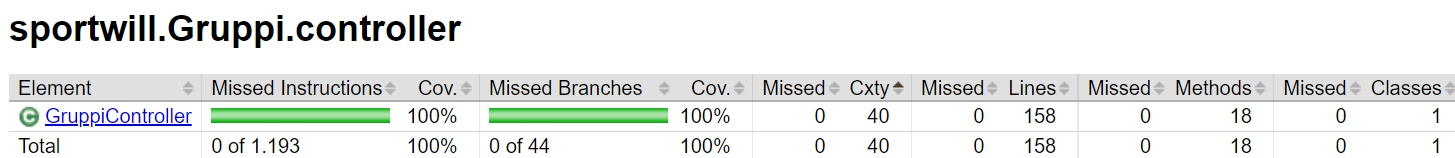
\includegraphics[scale=0.3]{verifica/coverage-gruppi-controller.jpg}}

    \caption{Code coverage della classe \texttt{GruppiController}}
    \label{img:code-coverage}
\end{figure}

\subsection{Test effettuati}

\begin{center}
  {\rowcolors{2}{color1}{color2}	    % rows height
    \renewcommand{\arraystretch}{1.60}
    \begin{longtable}{
      |>{\centering\arraybackslash}p{48pt}
      |>{\centering\arraybackslash}p{308pt}
      |>{\centering\arraybackslash}p{27pt}|}

      \rowcolor{antimaincolor!0}
      \caption{\label{tab:Test di unita}Test di unità}

      \\

      \hline
      % header
      \rowcolor{maincolor}
      % header color
      \color{antimaincolor}{Codice}
                  &
      \color{antimaincolor}{Descrizione}
                  &

      \color{antimaincolor}{Esito}

      \\
      \hline
      \endhead

      \hline
      % header
      \rowcolor{maincolor}
      % header color
      \color{antimaincolor}{Codice}
                  &
      \color{antimaincolor}{Descrizione}
                  &

      \color{antimaincolor}{Esito}

      \\
      \hline
      \endfoot

      TU1
                  & Il metodo \texttt{getAllGruppi}
      deve restituire tutti i gruppi presenti

                  & S                                              \\
      TU2
                  & Il metodo \texttt{getAllGruppi}
      deve restituire un \texttt{HttpStatus.NO\_CONTENT} nel caso non siano
      presenti
      gruppi
                  & S                                              \\
      TU3
                  & il metodo \texttt{getGruppo} deve
      restituire il gruppo specificato nel caso sia presente
                  & S                                              \\
      TU4
                  & il metodo \texttt{getGruppo} deve
      restituire un \texttt{HttpStatus.NO\_CONTENT} nel caso non sia presente
      il
      gruppo
                  & S                                              \\
      TU5
                  & Il metodo
      \texttt{getUtentiByGruppo} deve restituire gli utenti di un gruppo
                  & S                                              \\
      TU6
                  & il metodo \texttt{createGruppo}
      deve creare un gruppo
                  & S                                              \\
      TU7
                  & Il metodo \texttt{createGruppo}
      deve restituire un \texttt{ HttpStatus.BAD\_REQUEST} nel caso non esista
      il
      proprietario del gruppo specificato
                  & S                                              \\
      TU8
                  & Il metodo \texttt{createGruppo}
      deve restituire un \texttt{ HttpStatus.BAD\_REQUEST} nel caso che le
      coordinate
      geografiche inserite non siano valide
                  & S                                              \\
      TU9
                  & Il metodo \texttt{modifyGruppo}
      deve modificare un gruppo
                  & S                                              \\
      TU10
                  & Il metodo \texttt{modifyGruppo}
      deve restituire un \texttt{ HttpStatus.NOT\_MODIFIED} nel caso il gruppo
      specificato non esiste
                  & S                                              \\
      TU11
                  & Il metodo \texttt{modifyGruppo}
      deve restituire un \texttt{ HttpStatus.BAD\_REQUEST} nel caso non esista
      il
      proprietario del gruppo specificato
                  & S                                              \\
      TU12
                  & Il metodo \texttt{deleteGruppo}
      deve eliminare un gruppo
                  & S                                              \\
      TU13
                  & Il metodo \texttt{deleteGruppo}
      deve deve restituire un \texttt{ HttpStatus.BAD\_REQUEST} nel caso non
      esista
      il gruppo specificato
                  & S                                              \\
      TU14
                  & Il metodo
      \texttt{getUsciteByGruppo} deve restituire le uscite di un gruppo
                  & S                                              \\
      TU15
                  & Il metodo
      \texttt{getUsciteByGruppo} deve restituire un \texttt{
        HttpStatus.BAD\_REQUEST}
      nel caso non esista il gruppo specificato
                  & S                                              \\
      TU16
                  & Il metodo
      \texttt{getGruppiOfUtente} deve restituire i gruppi a cui partecipa un
      utente
                  & S                                              \\
      TU17
                  & Il metodo
      \texttt{addUtenteToGruppo} deve aggiungere un utente ad un gruppo
                  & S                                              \\
      TU18
                  & Il metodo
      \texttt{addUtenteToGruppo} non deve aggiungere un nuovo utente nel caso
      il
      gruppo abbia superato il numero massimo di utenti
                  & S                                              \\
      TU19
                  & Il metodo
      \texttt{addUtenteToGruppo} deve restituire un \texttt{
        HttpStatus.BAD\_REQUEST}
      nel caso non esista il gruppo specificato
                  & S                                              \\
      TU20
                  & Il metodo
      \texttt{removeUtenteFromGruppo} deve rimuovere un utente da un gruppo
                  & S                                              \\
      TU21
                  & Il metodo
      \texttt{removeUtenteFromGruppo} deve restituire un \texttt{
        HttpStatus.BAD\_REQUEST} nel caso non esista il gruppo specificato
                  & S                                              \\
      TU22
                  & Il metodo
      \texttt{deleteUtenteFromJointUtenteCrew} deve rimuovere un utente dalla
      tabella
      \texttt{joint\_utenti\_crew}
                  & S                                              \\
      TU23
                  & Il metodo
      \texttt{addUscitaToGruppoCrew} deve aggiungere un'uscita ad un gruppo
                  & S                                              \\
      TU24
                  & Il metodo
      \texttt{addUscitaToGruppoCrew}	deve restituire un
      \texttt{HttpStatus.BAD\_REQUEST} nel caso non esista l'uscita specificata
                  &
      S
      \\
      TU25
                  & Il metodo
      \texttt{addUscitaToGruppoCrew} deve restituire un
      \texttt{HttpStatus.BAD\_REQUEST} nel caso non esista il gruppo
      specificato &
      S
      \\
      TU26
                  & Il metodo
      \texttt{removeUscitaFromGruppo} deve rimuovere un'uscita dal gruppo
      specificato
                  & S                                              \\
      TU27
                  & Il metodo \texttt{removeUscitaFromGruppo} deve
      restituire un \texttt{HttpStatus.BAD\_REQUEST} nel caso non esista
      l'uscita
      specificata
                  & S                                              \\
      TU28
                  & Il metodo \texttt{removeUscitaFromGruppo} deve
      restituire un \texttt{HttpStatus.BAD\_REQUEST} nel caso non esista il
      gruppo
      specificato
                  & S                                              \\
      TU29
                  & Il metodo
      \texttt{deleteUscitaFromJointUscitaCrew} deve rimuovere un'uscita dal
      gruppo
      specificato
                  & S                                              \\
      TU30
                  & Il metodo
      \texttt{deleteUscitaFromJointUscitaCrew} deve restituire un
      \texttt{HttpStatus.BAD\_REQUEST} nel caso non esista l'uscita specificata
                  & S
      \\
      TU31
                  & Il metodo
      \texttt{deleteUscitaFromJointUscitaCrew} deve restituire un
      \texttt{HttpStatus.BAD\_REQUEST} nel caso non esista il gruppo
      specificato &
      S
      \\

    \end{longtable}
  }
\end{center}

% \section{Validazione e collaudo}             % Product Prototype
% !TEX encoding = UTF-8
% !TEX TS-program = pdflatex
% !TEX root = ../tesi.tex

%**************************************************************
\chapter{Conclusioni}
\label{cap:conclusioni}
%**************************************************************
%**************************************************************
\section{Raggiungimento degli obiettivi}
Sono stati raggiunti gli obiettivi fissati dello \textit{stage}. Inoltre, sono
stati portati a termine con un anticipo tale che ha reso possibile anche la
realizzazione di attività che non erano inizialmente pianificate.

\begin{center}
    {\rowcolors{2}{color1}{color2}
      \renewcommand{\arraystretch}{1}
      \begin{longtable}{
        |>{\centering\arraybackslash}p{60pt}
        |>{\centering\arraybackslash}p{220pt}
        |>{\centering\arraybackslash}p{60pt}|}
  
        \rowcolor{antimaincolor!0}
        \caption{\label{tab:raggiungimento-obbiettivi}Tabella raggiungimento degli obbiettivi}                                             \\
  
        \hline
        \rowcolor{maincolor}
        \color{antimaincolor}{Codice}                                                                 &
        \color{antimaincolor}{Descrizione}                                                               &
        \color{antimaincolor}{Esito}                                                                               \\
        \hline
        \endhead
  
        \rowcolor{maincolor}
        \color{antimaincolor}{Codice}                                                                 &
        \color{antimaincolor}{Descrizione}                                                               &
        \color{antimaincolor}{Esito}                                                                               \\
        \hline
        \endfoot
  
        O01     & Acquisizione competenze sulle tematiche sopra descritte & Soddisfatto \\
        \hline
        O02    & Capacità di raggiungere gli obiettivi richiesti in autonomia seguendo il cronoprogramma & Soddisfatto \\
        \hline
        O03     & Portare a termine l’implementazione dei \glspl{microservizio} richiesti con una percentuale di superamento pari al 80 & Soddisfatto \\
        \hline
        D01     & Portare a termine l’implementazione dei \glspl{microservizio} richiesti con una percentuale di superamento pari al 100 & Soddisfatto \\
        \hline
        D02     & Utilizzo della \gls{containerizzazione} per portare tutti i \glspl{microservizio} su Docker & Soddisfatto \\
        \hline
                
                                                                     
      \end{longtable}
      \renewcommand{\arraystretch}{1}
    }
  
  \end{center}

%**************************************************************
\section{Conoscenze acquisite}
Nel corso dello \textit{stage} ho appreso nuove tecnologie per la realizzazione
della parte sia \textit{back end} sia \textit{front end}. Tra le prime spiccano
l'utilizzo di Spring Boot e Spring Data JPA, oltre che i linguaggio Java. Ho,
infatti, avuto modo di conoscere uno  dei \gls{framework}  più importanti e
vasti per quanto concerne la programmazione in Java.\\
La conoscenza del linguaggio Java è sicuramente uno strumento molto utile per
la gestione della persistenza dei dati in un \textit{database} relazionale.
Combinando queste conoscenze con il \gls{framework} Spring è stato possibile
creare applicazioni \textit{Restful} in maniera semplice e veloce.\\
Per quanto riguarda il lato \textit{front end}, Angular utilizzato assieme al
linguaggio Typescript mi ha permesso di sviluppare in maniera efficiente ed
efficace attraverso le sue numerose funzionalità, tra cui \textit{templating},
\textit{two-way binding},
modularizzazione, gestione \gls{API} \textit{Restful} e \textit{dependency
    injection}.

%**************************************************************
\section{Valutazione personale}
Le aspettative sia mie che dell'azienda sono state ampiamente superate. Per
questo motivo, ritengo i risultati ottenuti nel corso dello \textit{stage} siano
sicuramente un successo, anche in virtù delle capacità acquisite. Quanto
prodotto ha migliorato il \textit{software} già in possesso all'azienda
e costituisce un punto di partenza per l'implementazione di nuove funzionalità.
Basterà infatti prendere spunto da quanto integrato nel corso dello
\textit{stage} per avere un'idea chiara su come implementare nuove
funzionalità. \\
L'utilizzo di due dei \gls{framework} più importanti e popolari per lo sviluppo
di applicazioni Java e per applicazioni \textit{web} dinamiche concorrono a
consolidare le mie conoscenze in Java e ad aggiungere al mio bagaglio di
conoscenze il linguaggio TypeScript.  \\
Infine, considero l'attività di \textit{stage} molto utile per capire come
funziona un'azienda e come ci si relaziona con i colleghi. Questo vale, in
particolare, per \myCompany: infatti, mi sono relazionato con lavoratori (e
colleghi) che si occupano di sviluppo di applicazioni usufruendo dei
\gls{framework} Spring e Angular.\\
Quanto vissuto in queste 8 settimane costituisce un'esperienza
preziosa per il mio futuro lavorativo e non.             % Product Design Freeze e SOP
\appendix                               
% !TEX encoding = UTF-8
% !TEX TS-program = pdflatex
% !TEX root = ../tesi.tex

%**************************************************************
\chapter{Appendice A}
%**************************************************************

\epigraph{Citazione}{Autore della citazione}             % Appendice A

%**************************************************************
% Materiale finale
%**************************************************************
\backmatter
\printglossaries
% !TEX encoding = UTF-8
% !TEX TS-program = pdflatex
% !TEX root = ../tesi.tex

%**************************************************************
% Bibliografia
%**************************************************************

\cleardoublepage
\chapter{Bibliografia}

\nocite{*}

% Stampa i riferimenti bibliografici
\printbibliography[heading=subbibliography,title={Riferimenti bibliografici},type=book]

% Stampa i siti web consultati
\printbibliography[heading=subbibliography,title={Siti web consultati},type=online]


\end{document}
